% =============================================================================================
% Trikaal — tokenizer study.  Build:  tectonic -X compile paper/main.tex
%
% DRAFT STATUS (2026-08-10)
%   §1–§5, §7, §8, Appendices A–E, References ... DRAFTED. Every number traced to a committed
%       artifact by an inline `% artifact:` comment (123 of them, 44 distinct paths).
%   §6  Results ........... STRUCTURED STUBS ONLY. No quantity in it exists until the
%       pre-registered run completes; each slot names the verdict-manifest field it binds to, so
%       filling it is a mechanical substitution. Both interpretation paragraphs are written and
%       dated 2026-08-10, before the run, so neither can be tuned to an outcome.
%   TITLE and ABSTRACT remain unlocked; two title variants are carried below.
%
%   Any \TBD{...} is a quantity that does not exist yet. No \TBD may be filled by estimate.
%   Any \PH{...} marks placeholder FIGURE data, which is implausible by construction per the
%   context-stripping rule — absent, symmetric about zero, or at an absurd magnitude.
% =============================================================================================
\documentclass[10pt]{article}
\usepackage{preprint}

% ---- TITLE: two candidates, neither locked until the legibility gate and verdict land -------
% (mechanism-led — current)
\title{Capacity Eviction in Reconstruction-Trained Tokenizers:\\
       A Controlled Study on Financial Microstructure}
% (ablation-led — alternate)
% \title{Does Microstructure Survive Tokenization?\\
%        A Pre-Registered, Capacity-Matched Ablation on Crypto K-Lines}

\author{Lakshay Bhati\\ \TBD{affiliation} \\ \texttt{\TBD{email}}}
\date{Preprint --- draft of \today}

\begin{document}
\maketitle

% --- ABSTRACT TRACEABILITY (strip before final) -----------------------------------------------
% Every number below is receipt-backed; the only unmeasured slot is \TBD{verdict}.
%   0.98 / 0.82--0.92 / 0.001--0.014, 3 seeds
%       runs_manifest/m6_interface_respec_design_pass.json ::
%       tokenizers.new_pointwise_fine_3seed.seeds.{0,1,2}.nonlinear_diagnostics
%         .point_decoder_per_dim_corrs
%       seed0 [0.9818, ..., 0.0140, ...] seed1 [0.9815, ..., 0.0011, ...] seed2 [0.9823, ..., 0.0053, ...]
%       dim 0 = return channel; dims 1--8,10--12 = correlated block (min 0.8235, max 0.9188);
%       dim 9 = the independent dimension.
%   1.151 nats   DERIVED: 0.5*ln(1+c^2) at c_signal = 3.0 (scripts/m6_canary.py C_SIGNAL);
%                prereg records the same quantity as "~1.15-nat plant" at docs/m6_prereg.md:2923.
%                Derivation shown in full at §3.3.
%   0.05 / 40    runs_manifest/m6_canary_v6_stage1_manifest.json ::
%                decision_inputs.{tf_corr_max = 0.0433, tf_flat_every_eval};
%                40 = recipe.budget_steps 20000 / recipe.eval_every 500.
%   0.900 nats   runs_manifest/m6_token_control_run_manifest.json ::
%                full_stream_receipts.exact_info_nats = 0.9002715667652758
%   94.4%        same :: decision_inputs.final_val_minus_H0 = -0.8496; 0.8496/0.90027 = 0.9437
%   0.5135       runs_manifest/m6_token_control_step0.json ::
%                id_visibility_probe.{logistic_sign_accuracy = 0.5135166645050049,
%                logistic_chance = 0.50}
%   0.9047 / 0.90  runs_manifest/m6_lambda_search_receipt.json ::
%                formal_cell_path_pin3_omp3.{mean = 0.9047, min = 0.8839, restated_gate_pass}
%   304,625,181 / 200  runs_manifest/m6_c15b_lake_surface_check.json :: bars, symbols
%   20.058 bpt (unchanged bits/token)  git show c4cd082:runs_manifest/
%                m6_interface_respec_design_pass.json ::
%                gate2_blocked_diagnosis.capacity_arithmetic.total_bpt_pinned
%   3.518 / 0.5 / 0.027  see the three comments at the end of this abstract.
% ----------------------------------------------------------------------------------------------
\begin{abstract}
Two-stage models for financial time series learn a tokenizer under a reconstruction objective
and then fit an autoregressive model to the resulting discrete codes. This design carries an
unstated assumption: that a representation good enough to reconstruct from is good enough to
forecast from. We show that it fails, and that it fails in a specific, predictable direction.
Reconstruction objectives allocate code capacity by variance and covariance and never by
downstream value, so wherever the code budget is tight enough that not every dimension can be
coded and the competing dimensions are correlated enough to amortize one another, a low-variance
channel that is weakly covariant with price --- which is what microstructure is --- is evicted
deterministically rather than by chance. On an
% The two conditions are carried here, not only in §3.1: an abstract is quoted without its section.
entropy-calibrated fixture in which every non-price dimension carries identical marginal
variance and differs only in cross-dimensional dependence, per-dimension reconstruction sorts
by variance class: $0.98$ for the high-variance return channel, $0.82$--$0.92$ for the
mutually correlated block, and $0.001$--$0.014$ for the one independent dimension, with the
ordering near-identical across three seeds. A signal worth $1.151$ nats planted in feature
space is not recovered at all (probe correlation below $0.05$ at all $40$ evaluations), while
$0.900$ nats planted directly in token space is recovered by the identical backbone at $94.4\%$
--- localizing the loss to the tokenizer--backbone interface rather than to model capacity. We
re-specify that interface so the fine subtoken is a per-bar encoding of the current bar,
restoring per-bar legibility from $0.5135$, against a chance rate of $0.50$, to $0.9047$ under a
gate pinned at $0.90$, and recovering the original feature-space signal at unchanged bits per
token. We then evaluate whether real
% 0.9047 is the measured seed mean; 0.90 is the gate. The two were conflated here as "0.90".
trade-flow imbalance survives this pipeline in a pre-registered, capacity-matched five-cell
ablation with a shuffled-microstructure placebo, on $304{,}625{,}181$ one-minute bars across
$200$ instruments, scored by cost-aware net information ratio: \TBD{verdict}. The design's
minimum detectable effect is $3.518$ annualized IR against a $0.5$ economic floor, and the only
prior we hold for the quantity under test is our own univariate screen of trade-flow imbalance on
a single symbol, $|\text{RankIC}| = 0.027$ at $h=5$ and $0.020$ at the headline horizon --- so a
null or inconclusive outcome is the most likely honest one. Both were pre-committed as publishable
before any result existed. Microstructure-awareness is an architectural property of a tokenizer,
not an emergent one.
% artifact: runs_manifest/m6_mde_inputs.json :: h15_pooled.MDE_annualized_IR = 3.518
% artifact: src/trikaal/eval/verdict.py :: ECON_FLOOR_IR = 0.5
% artifact: docs/milestone2_btcusdt_stage1.md — TFI RankIC -0.0270 [-0.0304,-0.0236] at h=5,
%   -0.0197 [-0.0230,-0.0166] at h=15, BTCUSDT only; that doc calls it "a univariate liveness
%   screen, not the headline test", so the abstract must not let it read as a market prior.
\end{abstract}

% =============================================================================================
\section{Introduction}
\label{sec:intro}
% =============================================================================================
% §1 body — the funnel, written last.
%
% Division of labour with §3: this section owns the STAKES and the SHAPE of the finding; §3 owns
% the mechanism itself. §1 must not restate §3's opening, which already gives the two-stage
% framing and the unstated assumption. What §1 adds is why the failure is not random, what makes
% it checkable, and what this artifact is and is not.
% =============================================================================================

A tokenizer is a lossy compressor, and something has to decide what it discards. In the two-stage
design now common for time series --- a tokenizer trained to reconstruct, then an autoregressive
model fitted to the resulting discrete codes --- that decision is made by a reconstruction
objective, and the forecaster that consumes the codes has no vote in it. The arrangement is
inherited from image and audio tokenization, where it is sound: there, reconstruction \emph{is} the
task, so an objective that preserves what reconstructs well preserves what matters. Carried into
forecasting, the same objective is being asked a question it was never given: not how much of the
input survives, but \emph{which parts}.

Those come apart in a specific and predictable way. Reconstruction error is an average over
dimensions, weighted by how much each contributes to that average, so a dimension is worth coding
in proportion to its variance and to the variance it can explain in others. A dimension that is
low-variance and weakly covariant with the rest is cheap to abandon: dropping it costs almost
nothing on the objective, and the bits it would have consumed buy real reductions elsewhere. Under
a tight enough budget the objective does not merely deprioritize such a dimension --- it excludes
it, and does so the same way across initializations, because the exclusion follows from the
statistics rather than from where optimization happens to land.

That profile is a description of microstructure. Trade-flow imbalance and its companions are small
relative to price movement, and their relationship to contemporaneous returns is weak enough that a
code can reconstruct the bar without them. A microstructure-aware forecaster therefore depends on
exactly the channels a reconstruction-trained tokenizer has the least reason to keep. The failure
is not that the tokenizer is bad; it is that it is good at the objective it was given.

The difficulty in establishing this on market data is that a negative result there has too many
explanations --- no signal, too little capacity, too short a schedule. We therefore measure it on a
constructed fixture where the answer is checkable: every non-price dimension carries identical
marginal variance, and they differ only in dependence structure, so any difference in what survives
is attributable to that one property. We then plant a signal of exactly computable information
content and ask whether an end-to-end pipeline recovers it. It does not. The step that turns that
into a diagnosis rather than another ambiguous negative is a control: the same backbone, at the
same budget, recovers a signal planted directly in \emph{token} space at $94.4\%$ while recovering
none of a larger signal planted in \emph{feature} space. Model capacity is acquitted by
construction, and the loss is localized to the interface between the two stages.

The remedy follows from the diagnosis and is an interface property rather than a matter of scale.
The original design produces both halves of each token from one contextual encoder, so a bar's own
state is smeared across the tokens of every later bar in the window --- the window reconstructs
while the per-bar symbol carries almost nothing. Making the fine half a function of the current bar
alone, and shaping it with an objective that weights the microstructure block as a class, restores
per-bar legibility from $0.5135$, against a chance rate of $0.50$, to $0.9047$ --- at unchanged
bits per token --- and recovers the signal that was previously lost. Because a fixture result need not
transfer, that property is then converted into a gate that must pass on real data, on every one of
the six live microstructure dimensions, before any second-stage expenditure is authorized.

Whether real trade-flow imbalance survives this pipeline and reaches a cost-aware trading decision
is a separate question, and the mechanism above does not answer it. We test it in a
pre-registered, capacity-matched five-cell ablation with a shuffled-microstructure placebo, on
$304{,}625{,}181$ one-minute bars across $200$ instruments. The decision rule, the thresholds, the
horizon, the cost model, the seed count and the trial enumeration were fixed before any of their
inputs existed. We state plainly what the arithmetic of that design implies: its minimum detectable
effect is far above the only prior we hold for the quantity under test, so a null or inconclusive
outcome is the most likely honest one, and it was pre-committed as publishable before any result
existed.

Two things this paper is not. It is not a foundation model: the backbone is a fixed measurement
instrument, held identical across every arm so that the quantizer and the input arm are the only
varied factors, trained on one venue at one frequency, with no transfer claim of any kind. And it
is not a trading result --- the cost-aware information ratio is the yardstick the ablation is
scored on, not a strategy we are advancing. The claim is about tokenizers.


\begin{figure}[t]
  \centering
  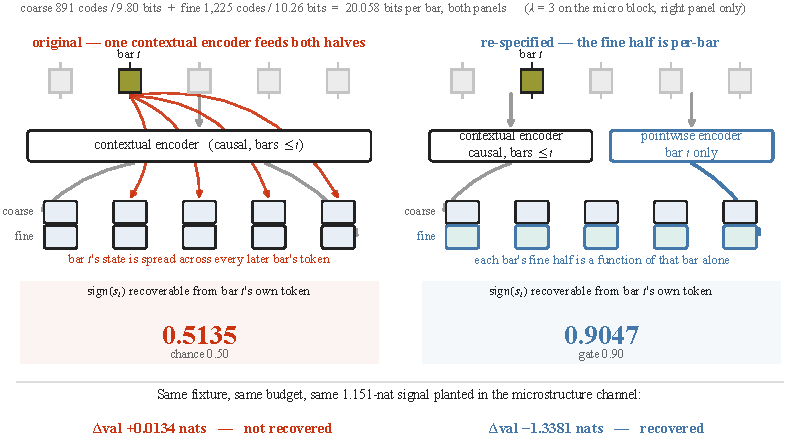
\includegraphics[width=\textwidth]{figures/fig1_mechanism.pdf}
  \caption{\textbf{One interface change decides whether a microstructure signal survives
  tokenization.} Each bar is encoded to a token pair --- a coarse and a fine subtoken, together
  $20.058$ bits --- which is what the autoregressive stage consumes. \textbf{Left, the original
  design:} a single causal encoder produces both halves. Because that encoder is contextual, bar
  $t$'s own state is distributed across the tokens of every later bar in the window, so the window
  reconstructs while the per-bar symbol carries almost nothing: the sign of bar $t$'s
  microstructure state is recoverable from bar $t$'s own token at $0.5135$, against a chance rate
  of $0.50$. \textbf{Right, the re-specified design:} the fine half is produced by a pointwise
  encoder that sees only the current bar, shaped by a per-bar bottleneck objective that weights the
  microstructure block as a class. Recoverability rises to $0.9047$ and is enforced thereafter by a
  gate at $0.90$. Bits per bar, the vocabulary split, the backbone and every evaluation instrument
  are identical between the two panels, so per-bar legibility is the only quantity that differs.
  What that difference buys downstream --- the same planted signal recovered on the right and not
  on the left --- is \cref{fig:extraction}; this panel is the interface, not the result.}
  % The Delta-val strip was removed 2026-08-10 (§3 review): Fig 3 owns the extraction result, and
  % two figures asserting the same result is one place for them to drift apart.
  \label{fig:mechanism}
\end{figure}

\paragraph{Contributions.}
\begin{itemize}[leftmargin=1.4em,itemsep=2pt,topsep=2pt]
  \item We identify and mechanistically characterize \emph{capacity eviction}: under a
    reconstruction objective, code capacity is allocated by variance and covariance and never by
    downstream value, so a task-relevant channel that is low-variance and weakly covariant is
    excluded deterministically. We isolate the effect with a fixture in which the evicted
    dimension and the retained ones differ in exactly one property --- statistical independence
    --- and show the exclusion reproduces across seeds (\cref{sec:mechanism}).
  \item We localize the failure by construction rather than by inference: the same backbone at
    the same budget recovers $94.4\%$ of a signal planted in token space and none of a
    larger signal planted in feature space, which acquits model capacity and indicts the
    tokenizer--backbone interface (\cref{sec:mech-localize}).
  \item We introduce a per-bar tokenizer interface --- a pointwise fine subtoken with a
    bottleneck decode leg and calibrated class weighting --- that restores per-bar legibility at
    unchanged bits per token, and a \emph{legibility gate} that enforces the property on real
    data as a pre-second-stage hard stop (\cref{sec:mech-fix,sec:mech-gate}).
  \item We run a pre-registered, capacity-matched five-cell ablation with a shuffled
    microstructure placebo on $304{,}625{,}181$ one-minute bars, scored by cost-aware
    net information ratio under purged walk-forward validation, with the decision rule, seed
    count and multiple-testing correction fixed before any result existed
    (\cref{sec:setup,sec:results}).
\end{itemize}

% =============================================================================================
% =============================================================================================
% §2 Related work. Four clusters, each closing on what this paper does differently.
%
% Every entry cited here had its metadata verified against the arXiv abstract page or the
% publisher record on 2026-08-10; refs.bib records which venue fields were confirmed and which
% were left in preprint form rather than guessed.
% =============================================================================================
\section{Related work}
\label{sec:related}

\subsection{Foundation models for time series, and for K-lines}
\label{sec:rel-foundation}

A line of recent work trains a single sequence model on large, heterogeneous collections of time
series and evaluates it zero-shot or with light adaptation. \citet{ansari2024chronos} discretize
scaled real values into a fixed token vocabulary and train a language model over the resulting
symbols; \citet{das2024timesfm} train a decoder-only model over patched inputs;
\citet{woo2024moirai} train across frequencies and domains with a unified objective. Upstream of
these, \citet{nie2023patchtst} established the patch-as-token treatment that much of the line
inherits. The shared premise is that a general representation of temporal structure transfers.

\citet{shi2025kronos} apply that premise to financial K-lines, and it is the design this paper
starts from: a tokenizer trained to reconstruct per-bar market features, followed by an
autoregressive model over the resulting discrete codes. We inherit the two-stage arrangement, the
backbone dimensions and much of the training and evaluation scaffolding, and we vary one thing.
Every component here is written from scratch; the parent's weights are not used, and no result in
this paper is a comparison against them.

We should be exact about what this artifact is, because the surrounding literature invites a
larger claim than we can support. This is not a foundation model. The backbone is a fixed,
$31{,}795{,}200$-parameter measurement instrument, held identical across every arm so that the
quantizer and input arm are the only varied factors. It is trained on one venue, one instrument
class and one frequency, and we make no transfer claim of any kind. The object under study is the
tokenizer.

\subsection{Discrete tokenization, and what its objective actually optimizes}
\label{sec:rel-tokenization}

Learned discrete representations descend from \citet{oord2017vqvae}, which pairs an encoder with a
learned codebook and a commitment loss. Two later families remove the codebook.
\citet{mentzer2024fsq} quantize each latent dimension to a small fixed set of levels, which
eliminates the codebook, the commitment term and codebook collapse together, at the cost of a
vocabulary that is a product of per-dimension level counts. \citet{zhao2024bsq} project to a
hypersphere and binarize, giving an implicit vocabulary exponential in dimension.
\citet{yu2024lfq} report that tokenizer design, rather than the generative model above it, is what
determines downstream quality --- a finding adjacent to ours in spirit and opposite in method,
since it is established by improving a tokenizer rather than by measuring what one discards.

The relevant observation for this paper is about evaluation rather than architecture. These
methods are compared on reconstruction fidelity, codebook utilization and downstream generation
quality, and the first of those is the objective they are trained on. That is appropriate where
reconstruction is the goal --- an image tokenizer that reconstructs well has done its job. It
becomes an assumption when the codes are handed to a forecaster, because the quantity that matters
downstream is not how much of the input survives but \emph{which parts} do. Reconstruction error
is an average over dimensions weighted by their contribution to that average, so a dimension can
be discarded almost entirely while the aggregate metric barely moves.

We are not aware of work that measures, for a reconstruction-trained tokenizer, which input
dimensions are preferentially discarded and whether the discarded ones are the task-relevant ones.
\Cref{sec:mechanism} is that measurement, on a fixture built so the answer is checkable, and
\cref{sec:mech-fix} is an interface that changes it.

\subsection{Microstructure as a predictive signal, and the distinction we are careful about}
\label{sec:rel-micro}

Order-flow imbalance is among the most robust short-horizon predictors in the microstructure
literature. \citet{cont2014ofi} show that price changes over short intervals are driven largely by
the imbalance between order-book events at the best quotes, a linear relationship with substantial
explanatory power. Related work reads informational content from the composition of flow rather
than its direction: \citet{easley2012vpin} construct a toxicity measure from volume-bucketed trade
imbalance and relate it to liquidity provision.

The distinction that governs this paper is that these are not one quantity. Order-flow imbalance
in the sense of \citet{cont2014ofi} is computed from \emph{order-book depth} --- the arrival,
cancellation and execution of resting liquidity at the best quotes. What we compute is signed
\emph{executed-volume} imbalance from aggregated trades, which requires no depth feed and is
available in the public dumps this study is built on. Trade signing itself has a literature
\citep{lee1991trade}; our source labels the aggressor side directly, so no signing heuristic is
applied and none of that literature's classification error enters our features.
% artifact: src/trikaal/data/reduce.py:75 — buy = pl.col("is_buyer_maker").not_(), i.e. taker BUY is
%   read from the exchange's own flag on each aggregated trade, not inferred from a quote rule.

We therefore use the name trade-flow imbalance throughout, in prose, configuration and code, and
never the order-flow name. This is not pedantry about terminology. The published effect sizes
belong to the depth-based quantity, they are not evidence about ours, and a negative result here
is evidence about trade-flow imbalance only. Order-book depth is explicit future work
(\cref{sec:lim-features}).

\subsection{Evaluation discipline}
\label{sec:rel-eval}

The methodological literature this paper leans on is concerned with a single failure: that a
sufficiently determined search over strategies will produce an impressive backtest from noise.
\citet{harvey2016crosssection} argue that the accumulated multiplicity of published cross-sectional
predictors demands a substantially raised significance bar, and that most published findings would
not survive one. \citet{bailey2014dsr} give the deflated Sharpe ratio, which discounts an observed
Sharpe by the number of trials it was selected from and by the non-normality of the return series.
\citet{lopezdeprado2018advances} supplies the sample-hygiene machinery --- purging, embargoing and
combinatorially purged cross-validation --- that keeps overlapping labels from leaking a training
window into its own evaluation.

Our design takes all four instruments: purged walk-forward with a measured embargo, a paired
moving-block bootstrap, a deflated Sharpe ratio against an enumerated trial count, and a
cost-aware net information ratio rather than a gross one. \Cref{sec:setup} specifies them.

What we add is not a new statistic but a procedural commitment. The deflated Sharpe ratio corrects
for a trial count, and the trial count is supplied by the researcher; nothing in the instrument
prevents an author from reporting a smaller one than they searched. Pre-registration is what makes
that number checkable, and it is rare in this literature. We fixed the decision rule, the
thresholds, the horizon, the cost, the seed count and the trial enumeration before any of their
inputs existed, published the amendment log with the direction of each change recorded before the
change was evaluated, and pre-committed a null as publishable. \Cref{sec:repro} describes the
machinery; \cref{sec:repro-defects} reports what it caught.

\subsection{Position}
\label{sec:rel-position}

Against that background this paper makes one claim. Reconstruction-trained tokenizers allocate
code capacity by variance and covariance and never by downstream value, so a task-relevant channel
that is low-variance and weakly covariant is excluded --- deterministically, under conditions
\cref{sec:mech-claim} states --- and microstructure is exactly such a channel. The remedy is an
interface property rather than a bigger model or a longer schedule. Whether the same effect governs
real trade-flow imbalance in a real market is a separate question, and it is the one
\cref{sec:setup} was pre-registered to answer.


% =============================================================================================
% =============================================================================================
% §3 — the mechanism.  Zero run dependency: every number here is already measured.
% Each figure/number carries its artifact in a % comment; strip the comments before submission.
% Floats: Figure 2 (eviction), Figure 3 (extraction). Figure 4 (legibility) is added at its
% production turn, anchored at the marked point in §3.7.
% =============================================================================================
\section{Capacity eviction in reconstruction-trained tokenizers}
\label{sec:mechanism}

Two-stage models for financial time series learn a tokenizer under a reconstruction objective and
then fit an autoregressive model to the resulting discrete codes
\citep{shi2025kronos,oord2017vqvae}. The design carries an assumption that is seldom stated: that
\emph{a representation good enough to reconstruct from is good enough to forecast from}. The
tokenizer is fitted to reconstruction, the forecaster never sees the underlying series, and nothing
in the pipeline is trained to preserve what the forecaster will need.

We show that the assumption fails, that it fails deterministically rather than by chance, and that
it fails hardest on precisely the channels a microstructure-aware model depends on. We state the
mechanism (\cref{sec:mech-claim}), measure it (\cref{sec:mech-measure}), test the prediction it
makes about an end-to-end pipeline (\cref{sec:mech-predict}), localize the loss by construction
rather than by inference (\cref{sec:mech-localize,sec:mech-interface}), give an intervention that
removes it (\cref{sec:mech-fix}), and convert the result into a standing gate that must pass on
real data before any second-stage expenditure (\cref{sec:mech-gate}). Every measurement in this
section is made on a synthetic fixture with a known ground-truth signal, chosen so that the
quantity being recovered is exactly computable; \cref{sec:mech-scope} states what that does and
does not license.

\subsection{The mechanism}
\label{sec:mech-claim}

A tokenizer maps each bar to a code of fixed size, so capacity is scarce and must be allocated
across the bar's dimensions. The allocation is chosen by whatever the objective rewards, and a
reconstruction objective rewards two things.

\begin{quote}
\textbf{Claim.} Under a reconstruction objective, code capacity is allocated in order of the loss
reduction each dimension buys. That ordering is set by a dimension's \emph{variance}, which bounds
how much loss it can contribute, and by its \emph{covariance} with dimensions already coded, which
determines how cheaply it can be served by capacity already spent. Downstream predictive value
enters nowhere. A dimension that is low-variance \emph{and} weakly covariant with the rest is
therefore the last claim on the budget. Where two conditions hold together --- a budget tight
enough that not every dimension can be coded, and competing dimensions correlated enough that
coding them is partly amortized --- that dimension receives nothing, and does so deterministically:
not occasionally, but in every run. Where either condition fails, the same objective still
allocates by the same rule, but the exclusion is no longer determined; \cref{sec:mech-measure}
reports a fixture in which the second condition is absent and the allocation is an initialization
lottery instead.
\end{quote}

The budget is tight, and the arithmetic says by how much. The canonical configuration uses
per-dimension levels $(11,9,9,7,7,5,5)$, split into a coarse subtoken of $11 \times 9 \times 9 =
891$ codes ($9.80$ bits) and a fine subtoken of $7 \times 7 \times 5 \times 5 = 1225$ codes
($10.26$ bits), for $20.058$ bits per bar; the binary-spherical arm \citep{zhao2024bsq} spends
$10+10$ bits for $20.000$.
% artifact: src/trikaal/constants.py :: FSQ_LEVELS, derive_coarse_fine, FSQ_V_C=891, FSQ_V_F=1225; bits = sum log2 L_i
Recovering the sign of a jointly-normal dimension at accuracy $a$ requires a correlation
$\rho = \cos\bigl(\pi(1-a)\bigr)$, so the $a = 0.90$ we will require costs at least
$-\tfrac12\log_2(1-\rho^2) = 1.69$ bits for that dimension alone by the Gaussian rate--distortion
bound, and more under any realizable scalar quantizer. Thirteen live dimensions at that fidelity
would need at least $22.0$ bits --- more than the entire per-bar budget, at any coarse/fine split.
% artifact: git show c4cd082:runs_manifest/m6_interface_respec_design_pass.json :: gate2_blocked_diagnosis.capacity_arithmetic.{sign_acc_0.9_requires_rho=0.951, fine_bits_available=10.26, total_bpt_pinned=20.058}
% RULING (2026-08-09). The receipt's 1.78 bits/dim and 23.1 bits are UNSOURCED and are not published:
% no derivation of either exists anywhere in the object database, they were hand-authored into a
% diagnosis block the producing script never constructs, and 1.78 contradicts its own sibling field.
% Evidence: scripts/m6_interface_respec.py contains no occurrence of 'bit', 'rho', 'log2', 'cos' or
% 'capacity' at ANY of its four revisions (c4cd082, 4a8fb48, e8d2a06, 7da3dc0) and its main() writes
% only the keys artifact/tokenizers/g_parity_new_layout/gates/wall_s, so gate2_blocked_diagnosis was
% added to the JSON by hand; a scan of all 1,781 objects (reachable + dangling) finds the arithmetic
% in exactly two blobs, the receipt itself and BUILD_RECORD prose restating it; 47 principled
% quantization / rate-distortion formulas were evaluated and none reproduces 1.78 to 2 d.p.; and
% inverting the Gaussian bound at 1.78 bits gives rho = 0.9567, i.e. sign accuracy 0.906, not the
% 0.90 that produced the receipt's own rho = 0.951. 23.1 is 13 x 1.78 and inherits the same defect.
% We publish 1.69 and 22.0, which ARE derivable from the committed constants (src/trikaal/constants.py
% FSQ_V_C=891, FSQ_V_F=1225), are strictly more conservative, and carry the identical conclusion.
% The receipt's companion fields 0.951, 10.26 and 20.058 are reproducible and are used as given.
% Same block, same defect: its prose "~4-5 winner dims at ~1.7-1.8 bits each" is also unsourced
% (10.2586/1.78 = 5.76); the figure and caption report the MEASURED 4 per seed instead
% (m6_interface_respec_design_pass.json :: gates.channel_receipt_non_gating.dims_ge_090_by_seed).
Not every dimension can be coded well. Something must be dropped, and the objective decides what.

This matters here because microstructure has exactly the profile the claim identifies. Trade-flow
imbalance and the aggregate trade-flow statistics are low-variance relative to returns and only
weakly covariant with price shape --- they carry information about the near future precisely
because they are \emph{not} a restatement of the recent past. A tokenizer trained to reconstruct
will therefore allocate capacity away from them by construction. This is not a defect of the
objective; it is the objective working correctly against a goal it was never given. It also means
that ``microstructure-aware'' has to be an architectural property of a tokenizer, and cannot be an
emergent one.

\subsection{Measuring the eviction}
\label{sec:mech-measure}

To measure the claim we need a fixture in which one dimension differs from the others in exactly
the property the claim names, and in nothing else. We construct a synthetic bar stream in which
every dimension is marginally standard normal --- so all of them contribute equally to a
variance-weighted loss --- and then make eleven of them mutually dependent while one, the
\emph{signal} dimension, is independent of everything.

The dependence is not chosen for convenience; it is calibrated to the real data. On $30$ symbols
and $3{,}895{,}808$ unmasked bars, the Gaussian-copula correlation log-determinant over the seven
non-microstructure dimensions is $-6.4819$, a per-dimension entropy deficit of $0.4631$ nats. The
fixture reproduces that deficit with a cross-dimension AR(1) chain at $\rho = 0.7993$, achieving
$0.462$ nats against a $0.05$-nat tolerance.
% artifact: runs_manifest/m6_interface_respec_design_pass.json :: filler_calibration.{lake_measurement.{copula_corr_logdet=-6.4819, per_dim_deficit_nats=0.4631, symbols=30, unmasked_bars=3895808, sample_seed=20260720}, filler_rho=0.7993, achieved_per_dim_deficit_nats=0.462, tolerance_nats=0.05, within_tolerance=true}
One further dimension, the return, is driven by the signal dimension at a two-bar lag and so
carries $3.15\times$ the marginal standard deviation of the rest: it is the high-variance channel,
and it is also the only dimension with downstream value in this fixture, since it is what a
forecaster would predict.

\Cref{fig:eviction} and \cref{tab:eviction} report, for three independently initialized tokenizers,
how well each dimension can be recovered from the bar's own code. The result sorts by variance
class and does not vary across seeds. The return is recovered at $0.98$. The eleven mutually
dependent dimensions are recovered at $0.82$--$0.92$, because one shared component serves all
eleven at once and the capacity spent on it is amortized eleven ways. The signal dimension --- same
marginal variance as any single filler, differing only in being independent --- is recovered at
$0.001$--$0.014$. It is not coded at all.

\begin{figure}[t]
  \centering
  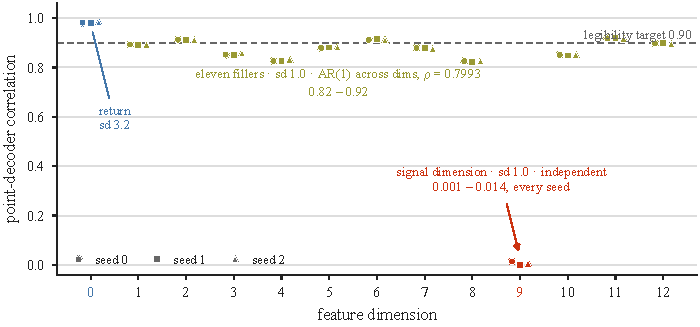
\includegraphics[width=\textwidth]{figures/fig2_eviction_by_variance_class.pdf}
  \caption{\textbf{Reconstruction quality is sorted by variance class, not by task relevance, and
  the ordering is deterministic.} Point-decoder correlation between each dimension's value at bar
  $t$ and its reconstruction from bar $t$'s own code, for three independently initialized
  tokenizers on a fixture whose non-signal structure is entropy-calibrated to the real data. The
  return dimension, whose marginal standard deviation is $3.15\times$ that of the others, is
  recovered at $0.98$; four of the thirteen dimensions clear the $0.90$ rule in every seed. The eleven filler dimensions, which have unit marginal variance and are coupled by an
  AR(1) chain across dimensions at $\rho = 0.7993$, are recovered at $0.82$--$0.92$. The signal
  dimension has \emph{the same unit marginal variance as the fillers} and differs from them in
  exactly one property --- it is statistically independent of everything --- and is recovered at
  $0.001$--$0.014$. The three seeds agree to within the marker width, so this is deterministic
  exclusion rather than an initialization lottery. Reconstruction objectives buy variance and
  covariance; they do not buy independence.}
  \label{fig:eviction}
\end{figure}

\begin{table}[t]
  \centering
  \small
  \caption{\textbf{Reconstruction quality by variance class, three seeds.} Point-decoder
  correlation between a dimension's true value at bar $t$ and its reconstruction from bar $t$'s own
  fine code. Every dimension except the return has unit marginal variance; the signal dimension
  differs from the fillers only in being statistically independent. Filler entries give the range
  over the eleven filler dimensions; per-dimension values are in \cref{app:eviction}.}
  \label{tab:eviction}
  \begin{tabular}{@{}llrrr@{}}
    \toprule
    dimension class & cross-dimensional structure & seed 0 & seed 1 & seed 2 \\
    \midrule
    return, sd $3.15$         & driven by the signal at lag 2            & $0.9818$ & $0.9815$ & $0.9823$ \\
    fillers ($11$), sd $1.00$ & AR(1) chain across dims, $\rho = 0.7993$ & $0.826$--$0.918$ & $0.824$--$0.919$ & $0.824$--$0.917$ \\
    signal, sd $1.00$         & independent                              & $\mathbf{0.0140}$ & $\mathbf{0.0011}$ & $\mathbf{0.0053}$ \\
    \bottomrule
  \end{tabular}
\end{table}
% artifact: runs_manifest/m6_interface_respec_design_pass.json :: tokenizers.new_pointwise_fine_3seed.seeds.{0,1,2}.nonlinear_diagnostics.point_decoder_per_dim_corrs
% marginal sd of the return: the receipt gives mean_baseline_mae 2.51351, and E|X| = sigma*sqrt(2/pi)
% => sigma = 3.1502, reported as 3.15 in figure, table and caption alike. The fixture's
% construction (scripts/m6_canary.py:229-234) gives sqrt(1+c^2) = sqrt(10) = 3.1623 exactly; we
% publish the receipt-supported finite-sample value, which is the smaller of the two.
% artifact: runs_manifest/m6_interface_respec_design_pass.json ::
%   gates.channel_receipt_non_gating.dims_ge_090_by_seed = {0: 4, 1: 4, 2: 4}

Calibrating the fixture to the real data is what makes this a mechanism rather than an anecdote,
and we report the correction it forced because it changes the strength of the claim. On an earlier
fixture whose dimensions were exchangeable i.i.d.\ draws --- no cross-dimensional dependence at all
--- the allocation was arbitrary: across three initializations the set of dimensions clearing $0.9$
changed completely, and the dimension of interest cleared in one seed of three.
% artifact: git show c4cd082:runs_manifest/m6_interface_respec_design_pass.json :: gate2_blocked_diagnosis.three_seed_winner_receipt (index 9: 0.91 / 0.26 / 0.10; note: tiny shells d64, 600 steps)
That reading makes the phenomenon an initialization lottery, which is a substantially weaker and
less actionable claim. Introducing the dependence structure the real data actually has replaced the
lottery with deterministic exclusion, because the correlated block then offers an amortization the
independent dimension cannot match.

\subsection{The prediction, tested}
\label{sec:mech-predict}

If a tokenizer evicts a channel then a signal carried only by that channel is unavailable to
everything downstream, however much information it contains and however capable the downstream
model is. We test that prediction by planting a signal of known size.

We build a three-symbol stream of $42{,}000{,}000$ bars. The signal dimension $s_t$ is drawn
i.i.d.\ standard normal and observed at the close of bar $t$; in the \emph{planted} arm it drives
the return two bars later,
\begin{equation}
  r_t \;=\; \sigma\bigl(\varepsilon_t + c\, s_{t-2}\bigr),
  \qquad c = 3, \quad \varepsilon_t \sim \mathcal{N}(0,1) \ \text{i.i.d.},
  \label{eq:plant}
\end{equation}
% artifact: scripts/m6_canary.py:220--247 (synth_symbol), C_SIGNAL=3.0, SIGNAL_LAG=2; runs_manifest/m6_canary_v6_stage1_manifest.json :: recipe.{bars_total=42000000, c_signal, signal_lag, sigma, symbols}
and in the \emph{noise} arm $s_t$ is redrawn independently, so the arms differ in exactly one
respect. Because the states are i.i.d., past returns reveal only states at lag $\geq 2$, which are
orthogonal to the forward label: the plant is recoverable \emph{only} through the microstructure
channel, and not through any function of price history.
% artifact: scripts/m6_canary.py:222--231 docstring — "causal AND asymmetric by construction"
Equation~\eqref{eq:plant} is a Gaussian channel, so the information it injects is exact,
\begin{equation}
  I\!\left(s_{t};\, r_{t+2}\right) \;=\; \tfrac12\ln\!\left(1+c^{2}\right)
  \;=\; \tfrac12\ln 10 \;=\; 1.151 \ \text{nats per bar},
  \label{eq:info}
\end{equation}
and because the tokens are a deterministic function of the features, the data-processing inequality
makes $1.151$ nats an upper bound on the validation cross-entropy improvement the autoregressive
stage can obtain from the plant.
% 1.151 = 0.5*ln(1+3^2) from receipt c_signal=3.0; the pre-registration records the same quantity at docs/m6_prereg.md:2923

Both arms were trained under an identical budget and schedule --- $20{,}000$ steps at batch $32$
and context $32$, giving $20{,}480{,}000$ bar-visits against a $27{,}300{,}000$-bar training region,
so $0.75$ epochs, and memorization is not available as an explanation. The sub-epoch condition is
asserted in the run receipt rather than assumed.
% artifact: same receipt :: sub_epoch.{bar_visits=20480000, train_bars=27300000, epochs_equivalent_train_region=0.7502, holds=true, rule}

The pipeline extracted none of it. The schedule completed on both arms with no loss spikes; the
validation--train gap was $+0.0072$ (noise) and $-0.0052$ (planted), confirming the sub-epoch
regime; the correlation between the model's forecast and the planted state stayed below $0.05$ at
\emph{every one of the $40$ evaluation points}, with a maximum of $0.0433$; and the planted arm's
final validation NLL was $13.6113$ against the noise arm's $13.5979$ --- worse by $0.0134$ nats,
which is the wrong sign.
% artifact: same receipt :: decision_inputs.{schedule_complete, lr_halved, gap_noise=0.0072, gap_planted=-0.0052, tf_corr_max=0.0433, tf_flat_every_eval, final_val_planted=13.6113, final_val_noise=13.5979, val_planted_minus_noise=0.0134}

The tokenizer was not discarding the state. Window-level reconstruction of the planted dimension
was non-degenerate in the same run: MAE $0.3044$ against a predict-the-mean baseline of $0.8216$.
% artifact: same receipt :: micro_recon["9"].{recon_mae=0.3044, mean_baseline_mae=0.8216, non_degenerate=true}
The information was present in the code stream and unavailable to the model consuming it.

\subsection{Localizing the loss: a token-space control}
\label{sec:mech-localize}

A null admits two explanations: the tokenizer's code geometry hides the rule, or the backbone
cannot learn thin conditionals at this scale. We separate them by construction rather than by
argument, planting a signal of comparable size \emph{directly in token space} --- bypassing the
tokenizer entirely --- and asking whether the same backbone at the same budget recovers it.

The plant redraws a target digit from a discretized Gaussian centred monotonically on a source
digit, with its width solved so the mutual information lands in a pre-registered band. It delivers
$0.9003$ nats exact over the full stream, agreeing with a Monte-Carlo plug-in estimate to
$2.0\times10^{-5}$, with a marginal KL of $0.0048$ and an entropy shift of $-0.005$ nats --- so no
information is smuggled in through the marginal --- and an unplanted control returns
$-8.8\times10^{-5}$. Construction, calibration, and the retirement of a first, information-poor
plant design are given in \cref{app:plant}.
% artifact: runs_manifest/m6_token_control_run_manifest.json :: full_stream_receipts.{exact_info_nats=0.9002715667652758, mc_plugin_info_nats=0.9002915157043878, closed_form_vs_mc_abs_diff=1.994893911205775e-05, target_marginal_kl_planted_vs_carrier=0.004795619186717248, entropy_shift=-0.005211528164841717}; runs_manifest/m6_token_control_step0.json :: plant_checks.unplanted_control_spearman=-8.759227241258484e-05
The carrier is the regenerated noise stream of \cref{sec:mech-predict} tokenized by that run's
frozen tokenizer, so token distribution, budget, schedule and validation protocol are unchanged,
and that run's noise arm supplies the reference $H_0 = 13.5979$.
% artifact: same :: recipe.carrier; decision_inputs.{H0_source, H0_val=13.5979}

The backbone recovers it almost completely: the probe crosses the pre-registered detection
threshold of $0.30$ at step $2{,}000$ and reaches $0.9999$, and the final validation NLL is
$12.7483$, that is $H_0 - 0.8496$ nats, or $94.4\%$ of the planted information.
% artifact: same :: decision_inputs.{probe_cross_step=2000, probe_final=0.9999, final_val_nll=12.7483, final_val_minus_H0=-0.8496}; 0.8496/0.9002715667652758 = 0.9437
\Cref{fig:extraction} places the two experiments side by side against their planted-information
references. The backbone is not the limiting factor. The loss is at the tokenizer--backbone
interface.

\begin{figure}[t]
  \centering
  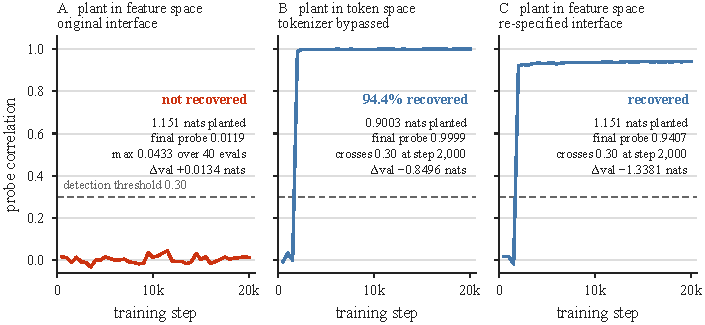
\includegraphics[width=\textwidth]{figures/fig3_extraction.pdf}
  \caption{\textbf{The same backbone extracts nearly everything from token space and nothing from
  feature space.} Nats of validation cross-entropy recovered against training step, measured
  against a matched reference run, with the dashed rule in each panel marking the information
  actually planted. \textbf{Left:} $1.151$ nats planted in feature space, where it must survive
  tokenization --- the curve never leaves zero, and the forecast--state probe stays below $0.05$ at
  all $40$ evaluation points. \textbf{Centre:} $0.9003$ nats planted directly in token space,
  bypassing the tokenizer --- the identical backbone at the identical budget recovers $0.8496$
  nats, $94.4\%$ of what was planted, crossing the detection threshold at step $2{,}000$.
  \textbf{Right:} the original feature-space plant, after the tokenizer interface is re-specified
  (\cref{sec:mech-fix}) --- recovery returns. Model capacity was never the constraint; the
  interface was.}
  \label{fig:extraction}
\end{figure}

\subsection{The interface defect, measured directly}
\label{sec:mech-interface}

The window encoder is causal but \emph{contextual}: bar $t$'s code is a function of bars
$\leq t$. State belonging to bar $t$ is therefore free to be distributed across the codes of every
subsequent bar in the window. The window as a whole reconstructs; no individual code need carry its
own bar's features. Since the autoregressive stage consumes exactly the per-bar code sequence,
anything that lives only in that spread-out form is unreachable.

The measurement is unambiguous. On $300{,}000$ bars of the planted stream, tokenized by the frozen
tokenizer of \cref{sec:mech-predict} with a $240{,}000/60{,}000$ split, a logistic probe recovering
$\operatorname{sign}(s_t)$ from bar $t$'s own coarse and fine digits achieves $0.5135$ against a
chance rate of $0.5$, and an MLP regressing $s_t$ on the same digits achieves a Pearson correlation
of $0.0142$ --- while the same tokenizer on the same stream reconstructs that dimension at the
window level at MAE $0.3044$ against a $0.8216$ baseline. The state is encoded, and per-bar
illegible.
% artifact: the 0.3044 / 0.8216 pair is NOT in the receipt below -- it is the window-level
%   reconstruction quoted 60 lines earlier, runs_manifest/m6_canary_v6_stage1_manifest.json ::
%   micro_recon["9"].{recon_mae=0.3044, mean_baseline_mae=0.8216, non_degenerate=true}.
% artifact: runs_manifest/m6_token_control_step0.json :: id_visibility_probe.{logistic_sign_accuracy=0.5135166645050049, logistic_chance=0.5, mlp_state_pearson_corr=0.014173370141830274, sample_bars=300000, train_test_split=[240000,60000], tokenizer, stream}

A stronger form of the same defect appears when the encoder is not causal at all, and we record it
because it is why causality is enforced. Perturbing only future bars inside a tokenization chunk
and counting how many past bars' tokens flip gives a leakage rate of $41.75\%$ coarse and $28.33\%$
fine on a tokenizer trained on real data; the causal-encoder control measures exactly $0.0\%$ on
both, which is what establishes that the probe can read zero.
% artifact: runs_manifest/m6_token_causality_probe.json :: results.trained_fsq_real_lake_smoke.{coarse_flip_rate=0.4175, fine_flip_rate=0.2833333333333333}; results.untrained_causal_flag.{coarse_flip_rate=0.0, fine_flip_rate=0.0}
Causal encoding is necessary for validity, and this section establishes that it is not sufficient
for usability: it removes the leak forward and leaves the smear backward.

\subsection{Intervention}
\label{sec:mech-fix}

If capacity is allocated by an objective that cannot see per-bar legibility, the remedy is to give
the objective a term that can. We make three changes. Each was necessary; none was sufficient
alone, and we report the intermediate failures because they are what establishes that.

\paragraph{(i) A pointwise fine encoder.}
The fine subtoken becomes a per-bar encoding of bar $t$'s own features, produced by a branch with
no cross-bar mixing, while the coarse subtoken retains the contextual causal encoder. Both
properties are carried in one token pair; bits per bar, the vocabulary split and the cell design
are untouched.
% src: src/trikaal/tokenizer/model.py:82--89 (PointwiseEncoder, w_in_fine), :136--144 (latent() overwrites the fine latent dims)
Alone this changed nothing --- legibility $0.5202$, at chance. The optimizer routed the state
through the contextual coarse smear and spent the fine bits elsewhere.
% artifact: git show c4cd082:runs_manifest/m6_interface_respec_design_pass.json :: gate2_blocked_diagnosis.iteration_history.iter1_pointwise_encoder_only

\paragraph{(ii) A per-bar bottleneck decode leg.}
A pointwise decode head must reconstruct bar $t$ from bar $t$'s fine code alone, with zero cross-bar
access, and its loss is added to the training objective.
% src: src/trikaal/tokenizer/model.py:96--102 (point_decoder), :230--236 (loss_point)
This trains --- the dimensions that win reach point-decoder correlation above $0.9$ --- but it does
not select \emph{which} dimensions win: legibility $0.5136$ and $0.5037$ at canonical width, and
$0.5014$, $0.4995$, $0.5182$ across three seeds on the entropy-calibrated fixture, a $3/3$ failure
against the $0.90$ threshold. That failure is the measurement plotted in \cref{fig:eviction}: the
leg works, and the objective still spends its budget on variance and covariance.
% artifact: git show c4cd082:... :: iteration_history.iter2_added_per_bar_bottleneck_leg; runs_manifest/m6_interface_respec_design_pass.json :: gates.gate2_legibility.{new_by_seed={0:0.5014,1:0.4995,2:0.5182}, threshold=0.9, pass=false, protocol}

\paragraph{(iii) Class weighting, with objective separation.}
The bottleneck loss weights the six microstructure dimensions as a class by a factor $\lambda$, and
the window reconstruction losses receive the fine channels detached, so the fine encoder is shaped
exclusively by the per-bar objective.
% src: src/trikaal/tokenizer/model.py:119--125 (w_feat_point), :207--217 (detach)
Detachment is load-bearing, and was measured to be: with the window loss attached the per-bar
weighting is inert at every $\lambda$ --- per-dimension receipts are identical from $\lambda = 2$
to $\lambda = 10^{6}$ --- because the window objective re-creates the smearing incentive as fast as
the leg removes it.
% artifact: runs_manifest/m6_lambda_search_receipt.json :: detach_amendment

$\lambda$ is calibrated, not chosen. Across $26$ trials no $(\lambda, \beta)$ pair cleared $0.90$
on all three seeds, which places the threshold inside the instrument's seed-noise band at the
achievable ceiling, while confirming that the state is carried (signal-dimension point-decoder
correlation $0.77$--$0.96$, microstructure class $0.86$--$0.92$, return preserved above $0.96$).
% artifact: runs_manifest/m6_lambda_search_receipt.json :: canonical_trials (26 entries), summary.finding
The acceptance rule was therefore restated over the three calibration seeds as mean $\geq 0.90$ and
every seed $\geq 0.85$, and $\lambda$ set to the smallest searched value clearing it: $\lambda = 2$
gives $(0.8365, 0.8594, 0.8592)$, mean $0.8517$ --- fail; $\lambda = 3$ gives
$(0.9060, 0.9142, 0.9000)$, mean $0.9067$, minimum $0.9000$ --- pass. Re-running through the pinned
construction path reproduces mean $0.9047$, minimum $0.8839$, bit-identically to the direct
construction at fixed thread count.

We state plainly that this is an acceptance threshold restated after seeing calibration results,
and why it is not the failure that description usually names. The restatement was forced by a
measured property of the instrument rather than chosen to admit a preferred value: $0.90$ sits
inside the calibration instrument's own seed-noise band of roughly $\pm 0.03$ at the achievable
ceiling, so a fixed single-seed threshold at exactly that value tests the noise as much as the
architecture, and the restated form --- a mean clause plus a per-seed floor --- is the standard
response to that situation rather than a loosening of it. It occurred entirely on the synthetic
calibration fixture, at a point when the real-data gate had never been executed and no real
microstructure had been tokenized. And it did not propagate: the standing gate that governs
expenditure (\cref{sec:mech-gate}) requires $\geq 0.90$ on \emph{every one} of the six
microstructure dimensions, with no mean clause and no floor, and nothing downstream of the
calibration was selected on the restated form.
% artifact: runs_manifest/m6_lambda_search_receipt.json :: seeded_campaign_omp2.{lam2,lam3}; pin.{PINNED_MICRO_POINT_WEIGHT=3.0, formula, lam2_seeded_fails}; formal_cell_path_pin3_omp3.{legibility=[0.9039,0.9262,0.8839], mean=0.9047, min=0.8839, restated_gate_pass=true}; path_determinism_proof
$\lambda = 3.0$ is pinned in the conformance surface, applies identically to both quantizers and
all input arms --- so it cannot differentially favour any cell --- and leaves bits per bar, the
cell matrix and every evaluation instrument unchanged.
% src: src/trikaal/eval/conformance.py:85,91,97 (PINNED_ENCODER_CAUSAL, PINNED_FINE_POINTWISE, PINNED_MICRO_POINT_WEIGHT)

\subsection{Verification, and the gate that carries it to real data}
\label{sec:mech-gate}

The intervention is verified by repeating \cref{sec:mech-predict} exactly: generator, seeds, stream
size, plant strength, lag, budget, schedule and validation protocol unchanged, the tokenizer
architecture the only difference.
% artifact: runs_manifest/m6_acceptance_stage1_manifest.json :: recipe.* — identical to the §3.3 receipt
The forecast--state correlation crosses the detection threshold at step $2{,}000$ and reaches
$0.9407$, with a maximum of $0.9414$. The planted arm's final validation NLL is $11.8478$ against
the noise arm's $13.1859$, a difference of $-1.3381$ nats where \cref{sec:mech-predict} gave
$+0.0134$; the schedule completes without spikes and both arms stay in the sub-epoch regime.
Per-bar legibility under the new tokenizer is $0.8990$ on the planted arm and $0.9084$ on the noise
arm, where \cref{sec:mech-interface} measured $0.5135$.
% artifact: same :: decision_inputs.{detect_cross_step=2000, tf_corr_final=0.9407, tf_corr_max=0.9414, final_val_planted=11.8478, final_val_noise=13.1859, val_planted_minus_noise=-1.3381, gap_noise=-0.0296, gap_planted=-0.1801, schedule_complete, branch='a_detect'}; runs.{planted,noise}.per_bar_id_legibility = 0.8989666666666667, 0.9084333333333333
We report $\Delta$val as the pre-registered decision statistic and not as an extraction fraction:
each arm trains its own tokenizer, so the arm difference is not calibrated against the $1.151$-nat
plant in the way \cref{sec:mech-localize}'s control is calibrated against its own $H_0$. \Cref{fig:legibility} places every stage of the intervention against the gate.
\begin{figure}[t]
  \centering
  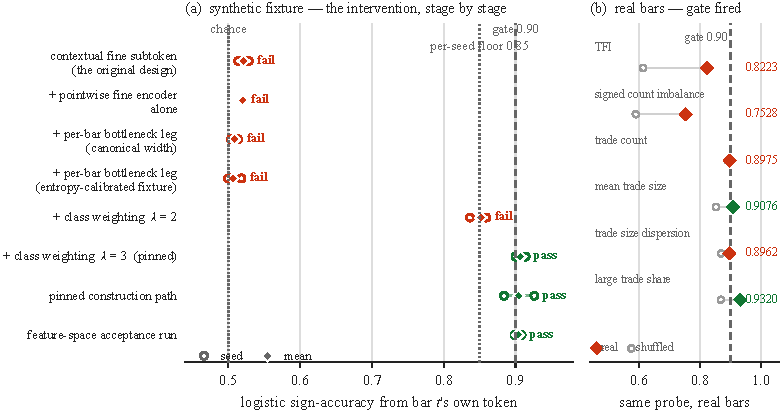
\includegraphics[width=\textwidth]{figures/fig4_legibility.pdf}
  \caption{\textbf{Only the third change moves per-bar legibility, and the threshold sits at the
  achievable ceiling.} \emph{Left:} logistic sign-accuracy of a microstructure dimension from bar
  $t$'s own token, across the intervention. Open circles are seeds and the diamond is their mean;
  the acceptance rule over the three calibration seeds --- \emph{restated} after seeing calibration
  results, as \cref{sec:mech-fix} sets out --- is mean $\geq 0.90$ and every seed $\geq 0.85$, so
  both thresholds are drawn. The original contextual design, the pointwise
  encoder alone, and the pointwise encoder with the bottleneck leg all sit at chance --- the leg
  trains, but does not decide which dimensions win. Class weighting at $\lambda = 2$ still fails;
  $\lambda = 3$ clears, and the pinned construction path reproduces it. Note how little headroom
  exists above the gate: this is the achievable ceiling, not a comfortable margin. \emph{Right:}
  the same probe applied to real microstructure by the standing gate, which ran after first-stage
  training and before any second-stage expenditure. \textbf{It fired.} Filled diamonds are the
  measured sign accuracies on real bars and open circles the same dimensions under the
  microstructure-shuffled placebo; the rule here is the gate's own, $0.90$ on \emph{every} live
  dimension with no mean clause, so both arms were refused. The shortfall is concentrated in the
  two signed channels, which are also the two that collapse under the shuffle while the four
  magnitude channels hold --- the ordering the mechanism predicts, on market data
  (\cref{sec:res-gate}).}
  \label{fig:legibility}
\end{figure}

% FIGURE 4 ANCHOR — per-bar legibility before/after with the 0.90 gate line is floated here at its
% production turn; the \cref{fig:legibility} reference is added to the sentence above at that time.

A mechanism established on a fixture is a hypothesis about the real data, so we convert it into a
gate rather than an expectation. After first-stage training and \emph{before any second-stage
expenditure}, each of the six microstructure dimensions must be linearly recoverable from bar $t$'s
own token pair at logistic sign-accuracy $\geq 0.90$ on the run's real training stream; failure
raises an exception and halts the run.
% src: src/trikaal/train/gates.py:96--97 (MICRO_DIMS=(7..12), MICRO_LEGIBILITY_MIN=0.9), :210--294 (micro_legibility_gate, RuntimeError)
The probe is a logistic regression on the one-hot digit decomposition of the coarse and fine codes,
trained for $300$ Adam steps at fixed seed on an $80/20$ split, deterministic given its inputs.
Sign accuracy is well defined for the magnitude-shaped dimensions because every microstructure
feature enters $z$-scored, so the sign is above-versus-below the causal rolling mean, and
per-dimension base rates are recorded so that residual class imbalance is visible. The sample is
stratified by symbol with the split blocked in time \emph{within} each symbol, which preserves both
properties that matter: full universe coverage, and no near-duplicate neighbours across the split.
% src: src/trikaal/train/gates.py:125--207 (id_legibility_sign_acc, _stratified_blocked_split), :223--230
Two defects in this gate were found and closed before it was relied upon, both of the form ``a
check that cannot fail is not a check''; they are documented with their fixes in
\cref{app:gate-defects}.

The gate's first execution on real microstructure is a named checkpoint with a pre-written
adjudication: if the real dimensions cannot clear the threshold under the calibrated architecture,
the run stops and reports with per-dimension receipts. It is not a threshold that may be moved.
% src: src/trikaal/train/gates.py:232--235
We record the expectation before the fact. Real trade-flow imbalance has the low-variance,
weakly-covariant profile that \cref{fig:eviction} shows being evicted, and the correction was
calibrated on a synthetic plant. \textbf{A gate failure on real data would be the real-data
confirmation of the mechanism} --- simultaneously a blocker for the ablation and the strongest
available evidence for the claim of \cref{sec:mech-claim}. Both outcomes are reportable, and
neither would be a surprise.

\subsection{Scope of the claim}
\label{sec:mech-scope}

Four limits, restated in \cref{sec:limitations}. First, everything above is measured on a
\emph{synthetic fixture}, not on real microstructure; the fixture's non-signal structure is
entropy-matched to the real data and its signal dimension is a controlled construction, which is
what makes the recovered quantity exactly computable and is also what stops it being a measurement
of markets. The mechanism is therefore not this paper's headline claim, and is not elevated to one
under any experimental outcome. Second, we demonstrate the effect for one reconstruction objective,
one quantizer family and one class of encoder: we show that \emph{this} objective allocates by
variance and covariance, not that no reconstruction objective can do otherwise --- and
\cref{sec:mech-fix} is itself a counterexample to the strong form, being a reconstruction objective
that carries the evicted channel because it was given an explicit term to do so. Third, the
$94.4\%$ of \cref{sec:mech-localize} is calibrated against a single matched reference run and
inherits whatever variation that run carries. Fourth, $\lambda$ is a hyperparameter fitted to a
synthetic proxy for the real allocation problem; it is pinned pre-data and applied identically
across every arm, so it cannot favour any cell, but the gate of \cref{sec:mech-gate} exists
precisely because the proxy might not transfer.


% =============================================================================================
% =============================================================================================
% §4 Experimental design. Zero run dependency: the design is frozen and every value below is a
% pin or a measurement that already exists. Artifact citations in % comments; strip before final.
% =============================================================================================
\section{Experimental design}
\label{sec:setup}

The mechanism of \cref{sec:mechanism} says that a reconstruction-trained tokenizer will evict
microstructure unless it is built not to. This section describes the experiment that asks the
separate question the paper is organized around: whether real trade-flow imbalance, carried through
a tokenizer built to preserve it, survives to a cost-aware trading decision. The design was frozen
before any of its numbers existed, and this section describes it as frozen.

\subsection{Five cells}
\label{sec:cells}

The experiment is a $2\times2$ over the two factors that could plausibly explain a difference ---
the quantizer and the input arm --- plus a fifth cell that isolates the one thing a $2\times2$
cannot: whether an effect attributed to microstructure is really microstructure.
\Cref{fig:design} shows the layout; the registry that the runner reads is the authority.
% artifact: src/trikaal/train/cells.py:40-44 — CellSpec(1,'bsq',ARM_OHLCV), (2,'fsq',ARM_OHLCV), (3,'bsq',ARM_MICRO), (4,'fsq',ARM_MICRO), (5,'fsq',ARM_MICRO_SHUFFLED)

Cells 1 and 2 receive the seven OHLC-shape, volume and amount dimensions only; cells 3 and 4
additionally receive the six microstructure dimensions (indices 7--12: trade-flow imbalance,
signed count imbalance, trade count, mean trade size, trade-size dispersion, large-trade share).
Cells 1 and 3 quantize with binary spherical quantization; cells 2 and 4 with finite scalar
quantization. Cell 5 is cell 4 with the microstructure block shuffled, and is the placebo.
% artifact: src/trikaal/constants.py :: OHLCV_ONLY_IDX = (0..6), MICRO_DIMS_IDX = (7..12), FEATURE_NAMES

The comparison that carries the paper is the paired difference $\Delta\IR(4-5)$. The others are
support: $\IR(4)-\IR(2)$ asks whether the microstructure arm beats the OHLCV arm without reference
to the placebo, and the two BSQ cells anchor the quantizer axis. We are explicit in
\cref{sec:limitations} that the three marginals involving a BSQ arm are withdrawn as claims,
because the BSQ implementation has no external reference point; they are reported, not claimed.

In the OHLCV-only arm the six microstructure dimensions are \emph{removed} from the input rather
than supplied and left uninformative, so that arm's feature width is seven rather than sixteen.
That choice matters for interpreting the legibility gate, which is undefined for an arm with no
microstructure channel and is exempted there by a named registry entry rather than by silence.
% src: src/trikaal/train/arms.py:49-59 — ARM_OHLCV: False with an explicit exemption reason string

\subsection{Capacity is controlled, not assumed}
\label{sec:parity}

A comparison between two quantizers is meaningless if one of them simply has more room. We
therefore control the two quantities that determine room, and report both rather than asserting
parity. The finite-scalar arm uses per-dimension levels $(11,9,9,7,7,5,5)$, split into a coarse
subtoken of $891$ codes and a fine subtoken of $1225$, for $20.058$ bits per bar; the
binary-spherical arm spends $10+10$ bits for $20.000$. The two differ by $0.058$ bits per bar,
inside a pre-registered parity band of $19.5$--$20.5$.
% artifact: runs_manifest/m6_interface_respec_design_pass.json :: g_parity_new_layout.{bpt_a=20.05784765541185, bpt_b=20.0}; src/trikaal/constants.py :: FSQ_BPT_BAND=(19.5,20.5)

The predictor realizes $31{,}795{,}200$ parameters at the finite-scalar vocabulary and
$31{,}725{,}568$ at the binary-spherical one. Of each, $10{,}493{,}952$ --- a third of the model
--- are the multi-token-prediction heads, which are trained and shipped; the backbone excluding
them is $21{,}301{,}248$ and $21{,}231{,}616$ respectively, and that is the figure the
construction gate pins. We quote both, and quote the total first, because the released weights
make the total checkable in one line and a reader who computes it should find our number. The two
arms differ by $69{,}632$ parameters --- $0.219\%$ of the realized model, equivalently $0.327\%$
of the backbone --- arising entirely from vocabulary-dependent embedding and output-head rows.
The heads are identical in both arms at $10{,}493{,}952$ each, so the gap is the same absolute
quantity on either basis. The backbone
is otherwise identical across all five cells: eight layers, model width $512$, feed-forward width
$1024$, eight heads, and a context of $512$ bars. It is held fixed on purpose. The tokenizer is
the object under study; the backbone is the instrument that measures it.
% artifact: THE COUNTS ARE CITED TO WHAT A READER CAN RECOMPUTE, not to an instruction document.
%   BSQ arm (the released weights): runs_manifest/m6_weights_release.json ::
%     units.{0,2,4}.predictor_parameter_groups.{n_params_realized_total = 31725568,
%     n_params_mtp = 10493952, backbone = 21231616}, and .how_to_verify prints the recipe --
%     "load predictor.pt and sum numel() over state_dict to reproduce n_params_realized_total".
%   FSQ arm: the released manifest does NOT carry 31,795,200, because the shipped units are cell 1
%     (BSQ). That figure is summed from runs_cloud/ckpt_cell4_seed0/predictor.pt and is asserted
%     at render time by paper/figures/make_fig5_design.py::_verify_params(), which raises on a
%     wrong constant and has been observed to do so.
%   The engineering-norms file remains the authority for the NORMS it states; it is not cited for
%   a measured quantity, because an instruction document ASSERTS a number where a manifest lets a
%   reader VERIFY one. Percentages computed here.

Every cell trains under the same budget: $26{,}003$ steps at batch $32$ and context $512$, on the
same draw. That budget is matched and fixed rather than chosen per cell by early stopping. The
alternative --- stopping each cell when its own validation loss saturates --- would give five
different budgets and confound $\Delta\IR(4-5)$ with ``cell 4 trained longer'', which is the same
class of confound the placebo exists to remove. The cost is that no cell is guaranteed to be at
its own optimum; saturation is measured and reported rather than optimized against.
% artifact: runs_manifest/m6_training_budget.json; docs/m6_design.md:18 (all cells share the training draw)

\subsection{The placebo, and the handicap it creates}
\label{sec:setup-placebo}
\label{sec:placebo}

The placebo answers a question no capacity control can: whether an effect attributed to
microstructure comes from microstructure's \emph{information} or merely from the model having six
more input channels to spend capacity on. Cell 5 receives the same six channels, with the same
marginal distributions, carrying no usable information.

The shuffle permutes the six microstructure dimensions as a block, within each contiguous segment
of a symbol, with a full within-segment permutation rather than a fixed block length. Three
properties are enforced rather than assumed. The block moves as a unit, so within-bar structure
\emph{among} the microstructure dimensions survives and only their relationship to everything else
is destroyed. The mask travels with the value, because permuting values alone would strand fill
values on valid bars and real values on masked ones --- a defect found in review and fixed before
any training. And the permutation is derived from the run seed and the symbol together, so the
train and evaluation paths shuffle identically.
% src: src/trikaal/eval/placebo.py — block permutation, cell5_seed(seed, symbol) = (seed << 16) ^ crc32(symbol)
% artifact: docs/BUILD_RECORD.md D6 — the (value, mask) pairing defect, closed 2cac96f

\Cref{fig:design} reports what the shuffle measurably does. It destroys the contemporaneous link
between microstructure and price shape, from mean absolute correlation $0.2037$ to $0.0005$, and
it destroys microstructure's own lag-1 autocorrelation, from $0.4165$ to $0.0006$. It leaves the
within-block correlation at $0.2886$ and the within-OHLCV correlation at $0.3105$, both unchanged.
% artifact: docs/m6_c12_placebo_mechanism.md — the four-row before/after table

This is where the design's principal known weakness lives, and we state it rather than let a
reader find it. Because cell 4's microstructure dimensions are correlated with price at $0.20$ and
autocorrelated at $0.42$, part of the capacity they consume is \emph{amortized} against structure
the code is already carrying. Shuffling removes that amortization along with the information, so
cell 5 pays a capacity price cell 4 does not. The consequence is a forfeit stated in the
pre-registered rule string itself: $\Delta\IR(4-5)$ is (information) $+$ (capacity handicap), and
the paper does not claim the information effect alone clears any threshold.
% artifact: src/trikaal/eval/verdict.py — clause 4 rule string names the composite quantity explicitly
The handicap is not quantified in information-ratio units, and \cref{sec:limitations} carries that
as an open disclosure rather than a resolved question.

\subsection{The headline metric, the geometry, and the decision rule}
\label{sec:metric}
\label{sec:geometry}
\label{sec:decision}

The headline is a cost-aware net information ratio, annualized, computed on a portfolio return
series. For a position of sign $s$ opened at the close of bar $t+1$ and closed $h$ bars later, the
realized net log-return subtracts execution and funding cost directly:
\begin{equation}
  r^{\text{net}} \;=\; s \log\!\frac{C_{t+h}}{C_{t+1}} \;-\; c_{\text{total}} \;-\; c_{\text{funding}},
  \qquad c_{\text{total}} = 2\,c_{\text{side}} .
  \label{eq:netret}
\end{equation}
A position is taken only where the forecast magnitude exceeds a threshold proportional to cost,
$\theta = \kappa c$, so the metric never rewards a forecast too small to pay for its own execution.
Entry at $t+1$'s close, not $t$'s, is the causal-safety margin: a decision made on bar $t$ cannot
transact at a price inside bar $t$. Information coefficient, rank information coefficient, mean
absolute error and $R^2$ are reported as diagnostics and none of them decides anything.
% artifact: src/trikaal/eval/harness.py — per-position net return; entry at t+1 close, exit at t+h;
%   theta = kappa * c_modeled per src/trikaal/eval/xsection.py:335.

Evaluation is purged walk-forward with an embargo, never a random split. The training region is
used once and never refitted; five forward blocks carry the headline; a $120$-bar embargo separates
each training window from the labels it must not see, built as the $60$-bar label look-forward plus
a $60$-bar serial-correlation margin. \Cref{sec:lim-embargo} reports the measurement that premise
rests on, including the channel where it does not hold.

\textbf{The decision rule was written, timestamped and committed before any cell was trained}, and
it is conjunctive: the primary outcome is \textsc{survives} only if none of five clauses fails, and
\textsc{null} otherwise. The clauses require, in order, that the one-sided $95\%$ lower bound of
$\Delta\IR(4-5)$ exceeds zero; that the effect reaches the paired minimum detectable effect, so an
effect too small for this design to resolve cannot be reported as one; that the lower bound of
$\IR(4)-\IR(2)$ exceeds zero, a comparison not involving the placebo at all, so a placebo pathology
cannot by itself produce a positive verdict; that $\Delta\IR(4-5)$ reaches an economic floor of
$0.5$ fixed before data, with the rule string naming the tested quantity as information plus
capacity handicap so the manifest cannot be read as claiming the information effect alone; and that
the deflated Sharpe ratio is at least $0.95$ over the enumerated trial set. \label{tab:verdict}
Two guards sit outside the clauses and are halt-only --- they can refuse to report an outcome their
inputs cannot support, and can never turn \textsc{survives} into \textsc{null} or the reverse.
\Cref{app:repro} gives the pinned constants, the exact clause strings, the trial enumeration, the
minimum-detectable-effect derivation and the guards' asymmetries; they are machinery, and a reader
does not need them to follow the result.
% artifact: src/trikaal/eval/verdict.py — clause keys 1_paired_ci, 2_mde_paired, 3_placebo_validity,
%   4_economic_floor, 5_dsr; ECON_FLOOR_IR = 0.5 defined :74, read :1074.

\textbf{The design's own arithmetic said the likely outcome was negative, and we recorded that
before running it.} The minimum detectable effect at the pinned horizon is $3.518$ annualized
information ratio; our prior for a univariate microstructure signal at that horizon is a rank
information coefficient of $0.0197$. On these numbers, \textsc{null} or \textsc{inconclusive} is
the most likely honest outcome, and \cref{sec:lim-power} states what that costs the design.

\subsection{Pre-registration as the integrity mechanism}
\label{sec:prereg}

Everything above --- the cells, the parity band, the placebo construction, the five clauses and
their thresholds, the horizon, the cost, the $\kappa$ grid, the seed count, the trial count and the
null basis --- is pinned on a conformance surface that the runner checks before it trains
anything, and each pin carries a mutation test proving the gate rejects its predecessor value.
Changing a pin is not a code edit that a reviewer must catch; it fails the run.
% artifact: src/trikaal/eval/conformance.py; per-pin mutation KATs

The pre-registration is a dated document with an append-only amendment log. Every amendment
records what changed, when, why, and --- where the direction was knowable --- whether it made the
bar easier or harder, recorded before the data that would reveal which. Amendments made after
seeing calibration results are marked as such, including the one described in
\cref{sec:mech-fix}. The log also contains withdrawn claims: statements this project made and
later retracted, retained rather than deleted. We regard that as the load-bearing part. A
pre-registration that only ever records successful predictions is not evidence of discipline; one
that records its own corrections is.
% artifact: docs/m6_prereg.md §7 — amendment log, entries v1.1 through v1.6.27, each dated


% The two figures belonging to §4. Held in their own file so that main.tex and review_s4.tex
% share one copy and the export cannot drift from the manuscript.
\begin{figure}[t]
  \centering
  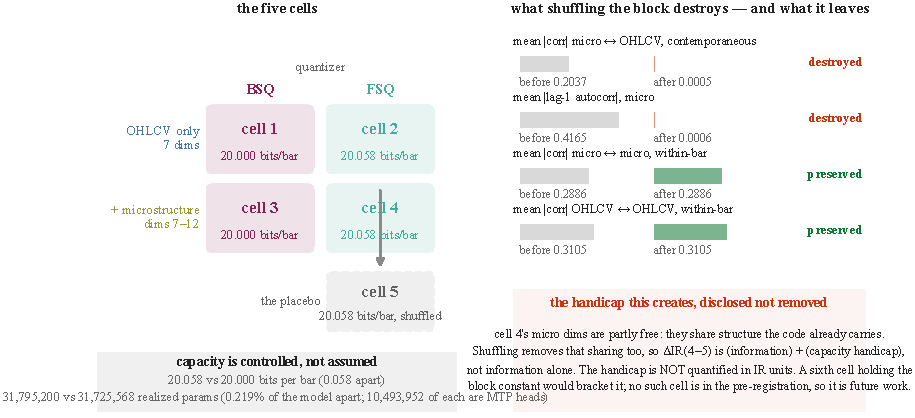
\includegraphics[width=\textwidth]{figures/fig5_design.pdf}
  \caption{\textbf{The five cells, at matched capacity, and the exact reach of the placebo.}
  \emph{Left:} a $2\times2$ over quantizer and input arm, plus a fifth cell that is cell 4 with the
  microstructure block shuffled. Capacity is controlled rather than assumed: the two quantizer arms
  differ by $0.058$ bits per bar and by $0.327\%$ of backbone parameters, so a difference between
  them cannot be attributed to one arm simply having more room. \emph{Right:} what the shuffle
  actually does, measured. It destroys the two things it was built to destroy --- microstructure's
  contemporaneous link to price ($0.2037 \rightarrow 0.0005$) and its own lag-1 autocorrelation
  ($0.4165 \rightarrow 0.0006$) --- and leaves the within-block and within-OHLCV correlations
  exactly as they were. The consequence is stated rather than hidden: because cell 4's
  microstructure dimensions are partly amortized against structure the code already carries,
  shuffling removes that sharing too, so $\Delta$IR(4$-$5) is (information) $+$ (capacity
  handicap). The handicap is not quantified in
  information-ratio units. A sixth cell holding the block constant would bracket it, but no such
  cell appears anywhere in the pre-registration, so it is future work rather than a committed
  contingency, and \cref{sec:limitations} carries the handicap as an open disclosure.}
  \label{fig:design}
\end{figure}
\clearpage
\begin{figure}[t]
  \centering
  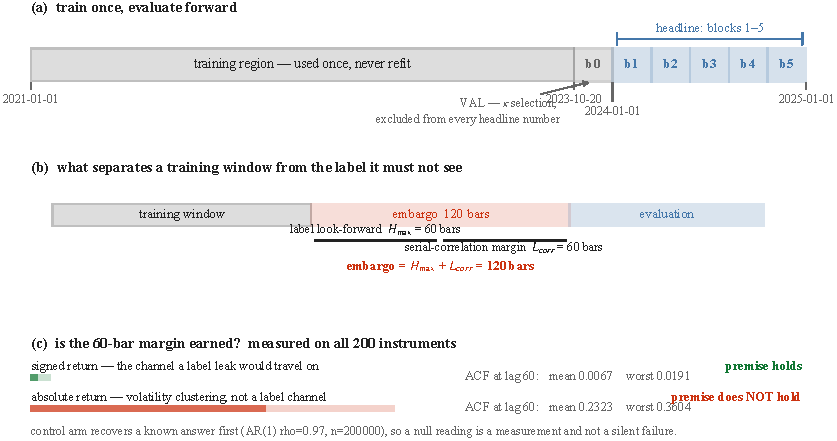
\includegraphics[width=\textwidth]{figures/fig6_validation.pdf}
  \caption{\textbf{Train once, evaluate forward, and pay for the separation.} \textbf{(a)} The training
  region ends at one boundary and is never refit. The forward region is cut into six blocks; block
  0 is spent selecting the execution filter and is excluded from every headline number, so the
  headline is scored on five blocks the selection never saw. \textbf{(b)} Between a training window
  and any label that could contaminate it sit a $60$-bar label look-forward and a $60$-bar
  serial-correlation margin, giving a $120$-bar embargo. \textbf{(c)} The premise behind that
  margin is measured on all $200$ instruments rather than assumed, and a control arm recovers a
  known AR(1) answer first, so a null reading is a measurement and not a silent failure. It holds
  for signed returns --- the channel a label leak would travel on --- at ACF $0.0067$ mean and
  $0.0191$ worst-symbol at lag $60$. It does \emph{not} hold for absolute returns
  ($0.2323$ mean, $0.3604$ worst), which is volatility clustering rather than a label channel;
  \cref{sec:limitations} carries that caveat.}
  \label{fig:validation}
\end{figure}

\clearpage

% =============================================================================================
% §5 Data.  Every number carries its artifact.
%
% The section's job is not to describe a dataset but to let a referee decide whether the dataset
% can support the claim -- so the ordering runs: what the universe is and why it is not
% survivorship-filtered, what a bar contains and what it does NOT, how normalization stays causal,
% what the quality gates cost, and what the experiment actually reads out of all of it.
% =============================================================================================
\section{Data}
\label{sec:data}

\subsection{One venue, and the universe chosen from inside it}
\label{sec:data-universe}

Every instrument is a USDT-margined perpetual future on Binance, sampled at one-minute frequency
over the four years \mbox{2021-01-01} to \mbox{2025-01-01}. Two public sources are combined per
bar: the klines dump supplies open, high, low, close, volume and quote volume; the aggregated-trades
dump supplies the signed trade statistics that the microstructure block is built from. No paid feed
and no order book is involved, which is a scope limit (\cref{sec:lim-features}) and also the reason
the corpus is reproducible by anyone.

The symbol set is bootstrapped \emph{from the data} rather than from the exchange's live instrument
list, and that choice is the one that decides whether the universe is survivorship-biased. A live
instrument listing contains only instruments that still exist; selecting from it silently deletes
every instrument that failed, which is the single most common way a backtest flatters itself. We
instead scan the S3 index of the aggregated-trades dumps once, which yields per symbol, without
downloading a single bar, the set of monthly dumps that exist. From that: the listing month is the
first dump, and an instrument is treated as delisted when its last dump trails the newest global
month. Ranking by total aggregated-trades bytes --- a liquidity proxy available from the same
index --- and taking the top 200 gives the universe: \textbf{200 symbols, of which 41 were already
delisted at the time of the scan}, each contributing only its $[\text{listing}, \text{delisting})$
bars.
% artifact: docs/milestone4b_universe_ingest.md §2 — dump-index bootstrap; "200 symbols selected, 41 delisted"; config/universe_full.yaml carries listing/delisting per symbol with a recorded config_hash

One detail in that rule is worth stating because it changes three symbols. A dump index is published
with lag, so an instrument that is merely a month behind the freshest global dump is not delisted ---
it is late. The delisting test therefore carries a one-month publish-lag tolerance, which corrected
three symbols relative to a zero-tolerance comparison. Without it the universe would have carried
three phantom delistings.
% artifact: docs/milestone4b_universe_ingest.md §2 and §7 — publish-lag tolerance, "corrected 3 symbols vs a zero-tolerance comparison"

The realized ingest is \textbf{304{,}625{,}181} bars across all 200 symbols. That is below the
$500$M--$1$B band the blueprint nominated, and we flag it rather than quietly re-describe the band:
200 instruments over the fullest available window, many of them partial-coverage through late
listing or delisting, lands near 300M. We regard it as adequate rather than merely acceptable, for
a reason that is about the model and not about the data --- a 21M-parameter backbone saturates
well below this, so the lake is bought for regime and cross-sectional breadth rather than as
training fuel. Reaching the nominal band would need roughly 320 instruments at proportional
bandwidth, and would not train a better model.
% artifact: runs_manifest/m6_c15b_lake_surface_check.json :: sampling.{bars = 304625181, symbols = 200, fraction_of_lake = 1.0, shards_sampled = ALL}
% artifact: docs/milestone4b_universe_ingest.md §4 exit-gate row — band flagged, corpus-purpose recorded in manifest metadata

\subsection{What a bar is, and what three of its dimensions are not}
\label{sec:data-features}

Each bar is reduced to a $16$-dimension feature vector. Seven dimensions are price shape and
liquidity: log close-to-close return, log range, body fraction, upper and lower wick fractions, log
volume and log quote volume. Six are the microstructure block, computed from aggregated trades:
trade-flow imbalance $(v_{\text{buy}} - v_{\text{sell}})/(v_{\text{buy}} + v_{\text{sell}})$,
signed count imbalance, log trade count, log mean trade size, trade-size dispersion, and large-trade
share. These six --- indices $7$ through $12$ --- are the block the ablation varies, and the first
of them is the quantity the paper is about.
% artifact: src/trikaal/constants.py :: FEATURE_NAMES (16 entries), MICRO_DIMS_IDX
% artifact: src/trikaal/data/features.py :: raw_feat[:, 7] = (v_buy - v_sell) / (v_agg + EPS_CNT), and rows 0--12 above it

The remaining three dimensions --- funding rate, log open interest and its change, indices $13$ to
$15$ --- are specified, wired through every transform, and \textbf{structurally absent}. The v1
ingest covers klines and aggregated trades only, so on all $304{,}625{,}181$ bars those three
columns have standard deviation exactly $0.0$ and their masks are set on $100\%$ of rows. We state
this here rather than in a footnote because the natural reading of ``a 16-dimensional
microstructure vector for perpetual futures'' is that funding and open interest are in it, and
they are not. The vector is $16$ wide and $13$ live. \Cref{sec:lim-features} carries what that
costs.
% artifact: docs/m6_prereg.md §7 v1.6.16 — x_13/14/15 stddev exactly 0.0, m_13/14/15 masked on 100% of bars
% artifact: src/trikaal/constants.py :: MASK_BITS_PERP = (13, 14, 15)

Every feature carries a companion mask bit, and the mask travels with the value through every
downstream transform. That pairing is not bookkeeping: a defect found in review had the placebo
shuffle permuting values while leaving masks in place, which would have stranded fill values on
valid bars and real values on masked ones. It was fixed before any training run.
% artifact: docs/BUILD_RECORD.md §2, D6 — "the placebo shuffle broke (value, mask) pairing"

\subsection{Normalization that cannot see forward}
\label{sec:data-causal}

Feature scales in this market move by orders of magnitude across four years, so the unbounded
dimensions are normalized rather than used raw. The normalization is where lookahead usually
enters a financial pipeline, through a statistic fitted on the whole sample and then applied to its
own training region, so the rule here is absolute: every statistic used for bar $t$ is computed
from data available at the close of bar $t$.

Nine dimensions --- the unbounded, scale-varying ones --- receive a causal exponentially weighted
z-score, at a half-life of $1{,}440$ bars (one day) for the fast group and $5{,}760$ bars (four
days) for the slow volume and open-interest group. Seven dimensions are already bounded or
relative, and are clipped only. Everything is clipped last to $[-5, +5]$ as an outlier guard. The
volatility scale $\sigma_t$ that the prediction targets are expressed in is built causally from
raw returns within a segment, on the same rule.
% artifact: src/trikaal/constants.py :: Z_SCORED_IDX (9 entries), BOUNDED_IDX (7), CLIP_LO/CLIP_HI = -5.0/+5.0, FAST_ZSCORE_IDX, SLOW_ZSCORE_IDX
% artifact: src/trikaal/data/config.py :: half_life_fast = 1440, half_life_slow = 5760; effective_n_warm(H) = max(n_warm, H//8); effective_n_warm_vol() = max(n_warm_vol, half_life_fast)

Each statistic needs a warm-up before it is trustworthy, and warmed-up bars are dropped rather than
back-filled. The cost is small and it is measured, not estimated: on the three thinnest instruments
in the universe the warm-up drop is $809$ of $279{,}930$ bars, $811$ and $809$ respectively ---
about $0.3\%$ --- because most instruments are long single segments and the warm-up is a one-time
tax at the start of each.
% artifact: docs/milestone4b_universe_ingest.md §4.1 spot-check — ZROUSDT 809/279,930 (0.3%), TURBOUSDT 811, NOTUSDT 809
% NOTE: that §4.1 prose calls this "the ~800-bar z-score warm-up", but the pinned constants give a
% 180-bar fast z warm-up, 720-bar slow, and 1,440-bar volatility warm-up (effective_n_warm_vol =
% max(30, 1440)), confirmed at runs_manifest/m6_c15b_lake_surface_check.json ::
% question_2....effective_n_warm_vol = 1440. The MEASURED drop of ~809 bars is what we quote; the
% "~800-bar warm-up" description is not reconciled with the constants and is not repeated here.

Causal safety is not asserted, it is a required continuous-integration gate. The test suite plants
lookahead leaks of several kinds --- a global one, a localized divisor leak, and a survivorship
leak in the target-validity flag --- and asserts that the exhaustive sweep catches each. One of
those tests exists specifically to show that a \emph{sampling} check misses the localized leak that
the exhaustive check catches, so the gate cannot be quietly weakened to a sampler. During ingest
the same sweep ran in-line on real cross-sections and a red result raised a fatal error before
anything was recorded.
% artifact: tests/data/test_causal_safety.py :: test_global_planted_leak_is_caught, test_localized_divisor_leak_caught_by_exhaustive_but_missed_by_sampler, test_localized_survivorship_leak_in_target_valid_is_caught, test_mask_is_strictly_causal
% artifact: docs/milestone4b_universe_ingest.md §6 — in-line sweep GREEN at scale on [live] HOOKUSDT, [tail] YFIIUSDT, [live] AXSUSDT; 100% coverage, 6,398 checks each; red raises FatalIngestError

\subsection{What the quality gates cost}
\label{sec:data-quality}

Of the $304{,}625{,}181$ bars, \textbf{$303{,}283{,}972$ ($99.56\%$) are usable by the OHLCV-only
arm} after warm-up and quality masking, and \textbf{$300{,}311{,}536$ ($98.58\%$) are usable by the
microstructure arms}. The ratio between those --- microstructure availability given price
availability --- is $99.0\%$ universe-wide, and no instrument falls below $0.7$. Across the
universe, $0.175\%$ of bars are stale and $0.376\%$ have zero volume.
% artifact: docs/milestone4b_universe_ingest.md §4.1 DQ table — total 304,625,181; OHLCV-usable 303,283,972 (99.56%); +micro-usable 300,311,536 (98.58%); micro-availability 99.0%, 0 symbols below 0.7; is_stale 0.175%, zero-vol 0.376%
% artifact: runs_manifest/m6_c10_micro_density.json :: symbols_with_zero_unmasked_per_dim = {} for dims 7--12; per_dim_total_unmasked ~ 3.0e8 each

That second number is the one that matters for the placebo. If microstructure were missing on a
large fraction of bars, cell 4 and cell 5 would differ in coverage as well as in content, and the
comparison the paper rests on would be confounded by absence rather than by information. At
$99.0\%$ availability with no starved instrument, it is not.

Forty-three instruments are thin, by a joint rule --- fewer than half the median usable bars, or
more than $10\%$ stale. Inspecting them rather than dropping them: almost all are recent 2024
listings with $280$k--$500$k bars and microstructure availability near $1.00$, so they are thin by
\emph{age}, not by quality. The single genuinely illiquid instrument is a delisted one at $2.5\%$
stale and $2.6\%$ zero-volume. All 43 remain in the lake; thinness is handled as a sampling weight
in the training draw, not as a deletion.
% artifact: docs/milestone4b_universe_ingest.md §4.1 — 43 thin-coin candidates, rule and per-symbol table at docs/_m4b_dq_table.md; FRONTUSDT stale 2.5% / zero-vol 2.6%

\subsection{Coverage, and the survivorship we did not remove}
\label{sec:data-coverage}

\Cref{fig:coverage} is the whole universe as a symbol-by-month raster: $7{,}024$ of a possible
$9{,}600$ symbol-months are present. The left staircase is instruments listing at different dates.
The right edge is ragged because instruments that stop trading are \emph{kept} in the lake, and
their absence afterwards is real absence rather than a filter. A survivorship-cleaned universe
renders as a solid rectangle, which is precisely the artefact the panel exists to demonstrate we
did not create. Two instruments have interior gaps rather than truncated tails and appear as
internal white streaks.

Two delisting counts appear in this project and they count different things, so we state both. The
ingest record's \textbf{41} is the number of instruments known to be delisted as of the index scan,
at any date. The \textbf{17} in \cref{fig:coverage} is the number whose data ends \emph{inside} the
four-year window, which is all a raster over that window can show; the remaining $24$ delist after
2024-12 and are complete here. The figure and this section therefore say ``stop trading inside the
window'' and never ``delisted''.
% artifact: paper/figures/make_fig7_coverage.py header — the 2026-08-09 reconciliation, spot-checked against the ingest note's own worked examples (AGIXUSDT, AUDIOUSDT); the note quotes the first ABSENT month, the lake stores the last PRESENT one
% artifact: coverage raster enumerated from processed/universe_bars/symbol=*/month=* at render time, 200 x 48

Survivorship is owned, not solved. Retaining failed instruments removes one bias; it does not
remove listing bias, since an instrument must have been listed on this venue at all to enter the
universe. \Cref{sec:lim-universe} carries that.

\subsection{Storage, provenance, and what makes a past prediction reconstructible}
\label{sec:data-provenance}

The reduced lake is Hive-partitioned Parquet under \texttt{(symbol, frequency, month)}, queried
through DuckDB. It was first written per-day, at $211{,}595$ files, which made per-symbol globbing
pathological; compaction to one file per symbol-month gives $7{,}024$ files and $15$\,GB. The
compaction was proven content-preserving rather than assumed: all $200$ per-symbol dataset hashes
were re-derived from the compacted lake and the universe Merkle root recomputed, with zero
mismatches and an unchanged root. Identical features, masks and timestamps imply an identical
causal result, so the hash comparison subsumes a re-run of the causal sweep.
% artifact: docs/milestone4b_universe_ingest.md §4.1 lake-compaction entry — 211,595 -> 7,024 files, 23 GB -> 15 GB, 0 hash mismatches, Merkle unchanged; scripts/compact_lake.py

Every dataset is content-hashed and the universe carries a single Merkle root over the lake,
\texttt{sha256:5dfd667d05b97bda\ldots}, recorded in the manifest alongside per-symbol listing and
delisting dates and a corpus-purpose note.
% artifact: docs/milestone4b_universe_ingest.md §4 — Universe Merkle sha256:5dfd667d05b97bda... (200-symbol; the 199-symbol first-pass intermediate was 9400a271...)

Raw dumps are not retained, and that is a deliberate position rather than a shortcut. The Merkle
root and the per-symbol hashes are taken over the \emph{reduced} lake, which is the artifact we
keep; the Binance SHA-256 of every raw shard is recorded for provenance only. Re-pulling raw and
re-running a deterministic reducer reproduces the recorded lake hash --- the reducer was proven
byte-identical at the preceding milestone --- so reproducibility survives eviction of $503$\,GB of
raw input.
\Cref{sec:repro} states exactly which parts of the pipeline are bit-exact and which are not.
% artifact: docs/milestone4b_universe_ingest.md §4.1 "Reproducibility survives raw eviction"; peak raw cache 30 GB, 503 GB cycled through eviction to raw 0

\subsection{What the experiment reads}
\label{sec:data-slice}

The lake is broader than the experiment. Of the $200$ instruments, the headline metric is scored on
$40$; the four-year window is split at its $0.7$ point, on 2023-10-20, into a training region and a
forward region, and the forward region is cut into six blocks of which block $0$ is spent selecting
the execution filter and excluded. The headline is therefore computed on blocks $1$ through $5$ ---
roughly 2024-01-01 to 2025-01-01, one year, $35{,}063$ stride-$15$ periods per instrument --- on a
region no selection step has seen. The other $160$ instruments and the preceding three years are
lake breadth and training data, not evaluation breadth, and \cref{sec:lim-universe} states what
that leaves unestablished.
% artifact: runs_manifest/m6_mde_inputs.json :: symbols_sampled (40 entries), primary_region_ms = [1704132000000, 1735689600000], n_blocks = 6, h15_pooled.T = 35063; conformance hard-asserts (val_block = 0, n_blocks = 6)


% The figure belonging to §5. Held in its own file so main.tex and review_s5.tex share one
% copy and the export cannot drift from the manuscript.
\begin{figure}[t]
  \centering
  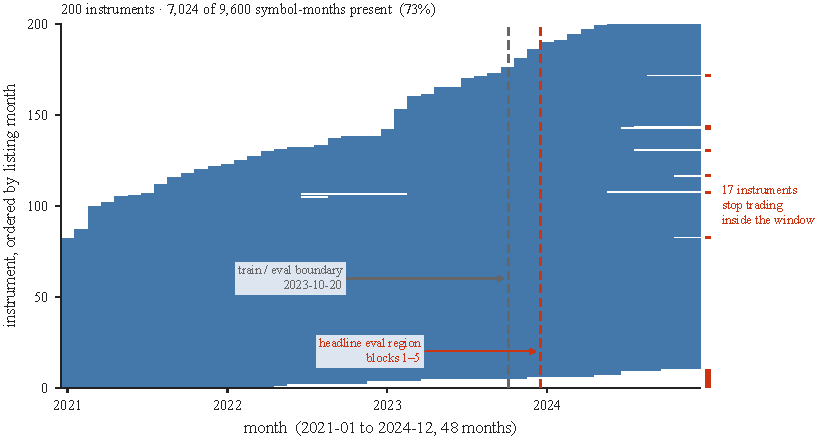
\includegraphics[width=\textwidth]{figures/fig7_coverage.pdf}
  \caption{\textbf{Survivorship is owned, not filtered away.} Month-by-month presence for all $200$
  instruments over the four-year window, ordered by listing month: $7{,}024$ of a possible
  $9{,}600$ symbol-months are present. The left staircase is instruments listing at different
  times; the right edge is ragged because instruments that stop trading are \emph{kept}, and $17$
  of them stop inside this window. A survivorship-filtered universe would render as a solid
  rectangle, which is the artefact this panel exists to show we did not create. Two instruments
  have interior gaps rather than truncated tails and appear as internal white streaks. The two
  dashed rules are the committed fold plan: training ends at the first, and the headline metric is
  scored only to the right of the second. Note that $17$ counts instruments whose data ends inside
  the window; the ingest record's $41$ counts every instrument known to be delisted at any date,
  including $24$ that delist after this window closes.}
  \label{fig:coverage}
\end{figure}

\clearpage

% =============================================================================================
% §6 Results — STRUCTURED STUBS ONLY. The pre-registered run has not been executed.
%
% CONTEXT-STRIPPING RULE (CLAUDE.md standing rules). Every slot below is \TBD{} or \PH{}, in red,
% and NO slot contains a plausible value. A reader who crops a paragraph out of this section must
% not be able to mistake any of it for a measurement. When the run lands, each \TBD is replaced
% from a single named field of the verdict manifest -- the field is named beside every slot so the
% substitution is mechanical and cannot be improvised.
%
% BOTH interpretation paragraphs in §6.6 are written NOW and dated, before any result exists, so
% that neither can be tuned to an outcome. That is the point of writing them here.
% =============================================================================================
\section{Results}
\label{sec:results}

\emph{The pre-registered run has not been executed. Every quantity in this section is an empty
slot bound to a named field of the verdict manifest, and every figure is drawn on placeholder data
that is implausible by construction. Nothing here is a measurement.}

\subsection{The pre-second-stage gate}
\label{sec:res-gate}

The legibility gate of \cref{sec:mech-gate} runs on real data before any second-stage training is
authorized, and it is a hard stop rather than a diagnostic: it requires at least $0.90$ sign
accuracy on \emph{every one} of the six live microstructure dimensions, with no mean clause and no
floor. Its outcome determines whether the rest of this section exists.

\begin{center}
\begin{tabular}{ll}
\toprule
quantity & value \\
\midrule
per-dimension sign accuracy, dims 7--12 & \TBD{six values} \\
minimum across the six & \TBD{min} \\
gate outcome & \TBD{pass or hard stop} \\
\bottomrule
\end{tabular}
\end{center}
% manifest binding: gates.gate2_legibility.{new_by_seed, min, threshold=0.90, pass}

\subsection{Primary outcome}
\label{sec:res-primary}

The five clauses of \cref{sec:decision} are evaluated conjunctively: the primary outcome is
\textsc{survives} only if none fails, and \textsc{null} otherwise. Two guards sit outside the
clauses and are \textsc{halt}-only. \Cref{fig:verdict} draws the surface.

\begin{center}
\begin{tabular}{lll}
\toprule
clause & tests & outcome \\
\midrule
1 paired CI & $\Delta\IR(4-5)$ lower bound $> 0$ & \TBD{} \\
2 MDE & $\Delta\IR(4-5) \ge$ paired MDE & \TBD{} \\
3 placebo validity & $\IR(4) - \IR(2)$ lower bound $> 0$ & \TBD{} \\
4 economic floor & materiality against the $0.5$ floor & \TBD{} \\
5 deflated Sharpe & against $SR_0$ at $N = 60$ trials & \TBD{} \\
\midrule
degeneracy guard & constant-direction book, any cell & \TBD{halt or clear} \\
power guard & across-seed range vs claimed effect & \TBD{halt or clear} \\
\midrule
\textbf{primary} & & \TBD{SURVIVES / NULL / INCONCLUSIVE} \\
\bottomrule
\end{tabular}
\end{center}
% manifest binding: clauses.{1_paired_ci, 2_mde_paired, 3_placebo_validity, 4_economic_floor,
% 5_dsr}.passed; degeneracy_guard.halted; power_guard.halted; primary. The rule STRINGS printed in
% Fig 8 are read from the manifest, not restated.

Both specifications required by the amendment window are reported from the same artifacts, and
their agreement or disagreement is stated here rather than in a footnote.

\begin{center}
\begin{tabular}{lll}
\toprule
 & v1.5 specification (primary) & retained alternative \\
\midrule
primary outcome & \TBD{} & \TBD{} \\
specifications agree & \multicolumn{2}{l}{\TBD{yes or no --- a first-class finding either way}} \\
\bottomrule
\end{tabular}
\end{center}
% manifest binding: dual_specification.* — a manifest lacking this field cannot be quoted (§7 v1.5)

\subsection{Effect sizes and secondary diagnostics}
\label{sec:res-effects}

Information coefficient, rank information coefficient, mean absolute error and $R^2$ are reported
as secondary diagnostics and do not enter the decision rule.

\begin{center}
\begin{tabular}{lccccc}
\toprule
cell & 1 BSQ/OHLCV & 2 FSQ/OHLCV & 3 BSQ/+micro & 4 FSQ/+micro & 5 placebo \\
\midrule
net IR, seed mean & \TBD{} & \TBD{} & \TBD{} & \TBD{} & \TBD{} \\
across-seed range & \TBD{} & \TBD{} & \TBD{} & \TBD{} & \TBD{} \\
RankIC & \TBD{} & \TBD{} & \TBD{} & \TBD{} & \TBD{} \\
decision activity at $\kappa^\ast$ & \TBD{} & \TBD{} & \TBD{} & \TBD{} & \TBD{} \\
\bottomrule
\end{tabular}
\end{center}
% manifest binding: per_cell.{ir_seed_mean, ir_range_across_seeds, rankic}; degeneracy_guard.
% per_cell.activity_decisions_seed_mean. The activity row is printed whatever it reads, per §4.4.

The three marginals involving a BSQ arm are reported and not claimed, for the reason
\cref{sec:lim-baseline} gives, and the required disclosure ships with them verbatim.

\subsection{Cost stress and seed dispersion}
\label{sec:res-stress}

\Cref{fig:cost} sweeps the round-trip cost around the pinned $0.30\%$; \cref{fig:seeds} plots each
cell's five seeds against the size of the effect being claimed. Both figures are built against the
manifest schema and are watermarked until the run lands.

\subsection{Interpretation}
\label{sec:res-interpretation}

\emph{Both paragraphs below were written on 2026-08-10, before the run was executed and before any
result existed. Exactly one will be retained; the other is deleted rather than softened. They are
placed here, in advance, so that neither can be written to fit an outcome.}

\paragraph{If the outcome is \textsc{survives}.} A positive $\Delta\IR(4-5)$ that clears the
paired confidence interval, the minimum detectable effect, the economic floor and the deflation
benchmark establishes that real trade-flow imbalance carries information beyond input capacity, and
that a tokenizer built to preserve it delivers that information to a cost-aware trading decision.
The claim ends there, and three limits bind it immediately. It is not a calibrated estimate of how
much: \cref{sec:lim-placebo} states that $\Delta\IR(4-5)$ mixes information with an unquantified
capacity handicap, so the measured difference is an upper bound on the information effect rather
than an estimate of it. It is not evidence that our BSQ baseline is competitive, so the
quantizer-axis marginals remain reported rather than claimed. And it is one exchange, one venue,
one instrument class and one year of scored data, with no regime-transfer test --- a positive
result here is an existence proof on this slice, not a property of markets. The mechanism of
\cref{sec:mechanism} would remain a fixture result; a positive outcome is consistent with it and
does not confirm it, because many differences between cells 2 and 4 could produce the same sign.

\paragraph{If the outcome is \textsc{null} or \textsc{inconclusive}.} This is the outcome the
design's own arithmetic makes most likely, and we pre-committed it as publishable before any result
existed, so it is reported without reframing. A null here means that under this pre-registered
decision rule, at this budget, on this slice, the microstructure arm did not beat its placebo by a
margin the design could resolve. It does \emph{not} mean microstructure carries no information: the
minimum detectable effect is $3.518$ annualized IR against a prior of $|\text{RankIC}| = 0.027$, so
the design would fail to detect a real effect of the size we actually expect, and
\cref{sec:lim-power} states that the effect we can detect is larger than the effect we predict.
Nor does it mean the mechanism of \cref{sec:mechanism} is wrong --- the mechanism is established on
a fixture and is not contingent on this outcome. What a null does establish is narrower and still
worth publishing: that the pipeline, with the interface defect removed and the legibility gate
passed, does not convert this microstructure signal into net information ratio at this scale.
Given how much of this literature reports only positive results, a pre-registered null with its
power analysis stated in advance is a contribution to the record rather than a failed experiment.
\Cref{sec:lim-power} names what would change the answer: more scored data, a lower-cost venue, or
an effect larger than our own prior.


% The three figures belonging to §6. Held in their own file so main.tex and review_s6.tex
% share one copy and the export cannot drift from the manuscript.
\begin{figure}[t]
  \centering
  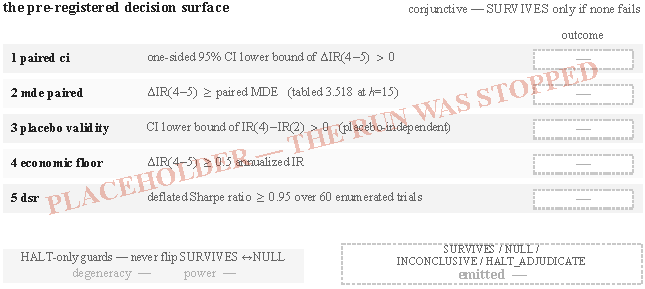
\includegraphics[width=\textwidth]{figures/fig8_verdict.pdf}
  \caption{\textbf{The decision surface, fixed before any result existed.} Five clauses, evaluated
  conjunctively: the primary outcome is SURVIVES only if none fails, and NULL otherwise. Two
  guards sit outside the clauses and are HALT-only --- they can refuse to report an outcome their
  own inputs cannot support, and can never flip SURVIVES to NULL or back. The rule strings shown
  are transcribed into this figure's source rather than loaded from a manifest, and are therefore a
  restatement; the persisted strings are the authority. \PH{no values} --- every outcome
  cell is empty because the run has not been executed; each is filled from a single named field of
  that manifest.}
  \label{fig:verdict}
\end{figure}
\clearpage
\begin{figure}[t]
  \centering
  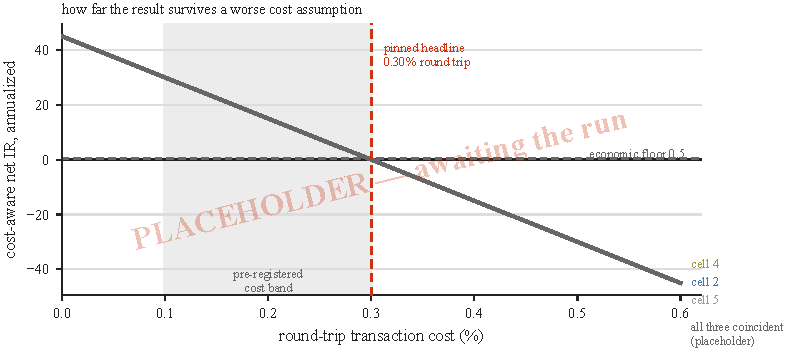
\includegraphics[width=\textwidth]{figures/fig9_cost_stress.pdf}
  \caption{\textbf{The specified cost-stress apparatus, with no curve.} Cost-aware net information
  ratio against the round-trip transaction cost was to be drawn here for the microstructure arm,
  the OHLCV-only arm and the placebo; the headline is pinned at $0.30\%$, the pessimistic end of
  the pre-registered $0.1$--$0.3\%$ band. \PH{no curve drawn} --- the ablation this panel was
  specified for never ran, so the axes, the pinned rate, the band and the economic floor are real
  and no cell is drawn. An earlier draft carried a placeholder line whose zero crossing fell
  \emph{exactly} on the pinned $0.30\%$ rule, the most quotable point on the axis; cropped away
  from this caption it read as a break-even of $0.30\%$, against a measured $0.0023$--$0.0208\%$.
  The one break-even we have measured is drawn instead, in red at the left margin, with its
  cell-1-only scope written into the image rather than left to the caption.}
  \label{fig:cost}
\end{figure}
\clearpage
\begin{figure}[t]
  \centering
  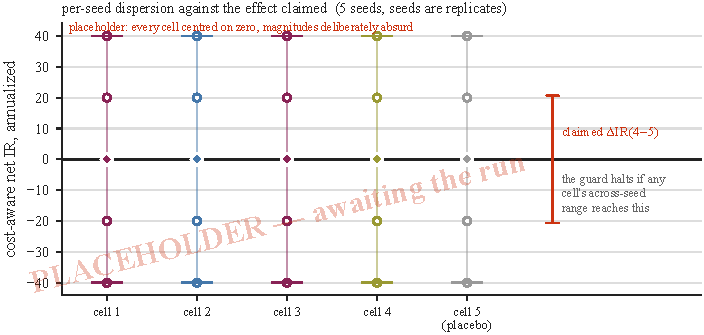
\includegraphics[width=\textwidth]{figures/fig10_seed_stability.pdf}
  \caption{\textbf{Seed dispersion against the effect being claimed.} Each cell's five seeds are
  replicates of one configuration, not five configurations; open circles are seeds, the diamond is
  the seed mean, and the bars mark the across-seed range. The comparison that matters is the one
  drawn on the right: if any cell's across-seed range reaches the size of the effect being claimed,
  the power guard halts and the verdict is reported as adjudication-required rather than as an
  outcome.
  \PH{every cell centred on zero, magnitudes $\sim\pm40$} --- no cell is favoured and the claimed
  effect is drawn symmetric about zero, so the panel shows the comparison's geometry and no
  result.}
  \label{fig:seeds}
\end{figure}
\clearpage


% =============================================================================================
% §7 Limitations.  Ordered by what a referee would attack first, not chronologically.
% Every number carries its artifact.  Nothing here is hedged into vagueness: a limitation stated
% imprecisely is not a disclosure.
% =============================================================================================
\section{Limitations}
\label{sec:limitations}

The limitations below are stated at the same confidence as the contributions, and in the order a
sceptical reader should apply them. Three of them --- the synthetic basis of the mechanism, the
absent external baseline, and the placebo's capacity confound --- bound what the paper is entitled
to claim even if every pre-registered clause passes.

\subsection{The mechanism is measured on a synthetic fixture, not on markets}
\label{sec:lim-fixture}

Everything in \cref{sec:mechanism} is measured on a constructed fixture. That is a deliberate
trade and it cuts both ways. The fixture's non-signal structure is entropy-matched to the real
lake --- a per-dimension deficit of $0.4631$ nats, reproduced at $0.462$ against a declared
tolerance of $0.05$ --- and its signal dimension is planted with an exactly computable information
content, which is what allows us to say that $94.4\%$ of a known quantity was recovered rather
than that a loss curve moved.
% artifact: runs_manifest/m6_interface_respec_design_pass.json :: filler_calibration.{lake_measurement.per_dim_deficit_nats=0.4631, achieved_per_dim_deficit_nats=0.462, tolerance_nats=0.05, within_tolerance=true}
It is also precisely what stops the result being a measurement of markets. We do not know the
variance and covariance geometry of real trade-flow imbalance against real price well enough to
assert that the fixture reproduces it; we know only that one entropy statistic matches.

The consequence is a specific one, and we hold to it under every experimental outcome: capacity
eviction is a mechanism we demonstrate, not a market phenomenon we measure, and it is not this
paper's headline claim. A reader who wants the mechanism established on real microstructure will
not find it here. What the pre-registered ablation of \cref{sec:setup} tests is the downstream
question --- whether real trade-flow imbalance survives the re-specified pipeline --- and a
positive result there would be consistent with the mechanism without confirming it, because many
other differences between cells 2 and 4 could produce the same sign.

Two narrower limits inside the same fixture. We demonstrate the effect for one reconstruction
objective, one quantizer family and one class of encoder. We show that \emph{this} objective
allocates by variance and covariance; we do not show that no reconstruction objective can do
otherwise, and \cref{sec:mech-fix} is a counterexample to the strong form --- it is a
reconstruction objective that carries the evicted channel, because it was given an explicit term
to do so. Separately, the $94.4\%$ recovery figure is calibrated against a single matched
reference run and inherits whatever run-to-run variation that reference carries; we report it as
one measurement, not as an expectation over runs.
% artifact: runs_manifest/m6_token_control_run_manifest.json :: decision_inputs.{H0_source, H0_val=13.5979, final_val_minus_H0=-0.8496}

\subsection{The BSQ baseline is ours, and nothing external anchors it}
\label{sec:lim-baseline}

Cell 1 --- binary spherical quantization on OHLCV-only inputs --- is our own implementation at
matched bits per token. It is not an independently validated reference. The evaluation harness was
originally specified to load published reference weights and reproduce their reported rank
information coefficient as an external anchor for this cell. That gate was found unexecutable and
dropped as binding before any cell was scored, for three separate reasons, each sufficient on its
own: the reference paper publishes two rank information coefficients for the same model that
differ by $2.4\times$ ($0.0431$ against $0.0665$) without the pre-registration saying which
applies; both are measured on Shanghai Stock Exchange $15$-minute equity bars, a market and a
frequency this study firewalls out of v1, so the gate's two requirements --- reproduce the
published number, and do it on our own pinned slice --- cannot both hold; and executing the
weights would require importing the reference model code, which our independence invariant
forbids. Resolvability was never the obstacle: the band is $4.51$ to $11.05$ standard errors wide
at the measured effective sample size of $1{,}401{,}637$.
% artifact: src/trikaal/eval/external_validation.py :: GATE_IS_BINDING = False, and the three-count comment above it
% artifact: runs_manifest/m6_c4_resolvability.json :: which_published_figure.{ic_price_series=0.0431, ic_return_forecasting=0.0665, dataset_in_the_caption}; resolvability_MEASURED.{n_eff_summed=1401637, se_rankic=0.0008446, band_over_se_price_series=4.51, band_over_se_return_forecast=11.05}

Two compensating controls were armed in its place, and it is important to be exact about what they
do. A saturation check asks whether cell 1 was trained enough to be a fair baseline. A codebook
utilization gate, pinned at $0.95$, asks whether our BSQ codebook collapsed. Neither answers the
question the external gate was for. We therefore carry the following sentence as a required field
of every verdict manifest, refused if absent, and reproduce it verbatim here:

\begin{quote}
We therefore cannot exclude that our BSQ baseline is weaker than a reference BSQ implementation,
which would inflate the FSQ-vs-BSQ comparison reported in \cref{sec:results}.
\end{quote}
% artifact: src/trikaal/eval/external_validation.py :: BSQ_DISCLOSURE (verbatim); conformance PINNED_CODEBOOK_MIN_UTILIZATION = 0.95

This bounds the quantizer leg specifically. It does not bound the input-arm leg: the comparison
between cells 2 and 4, and between cell 4 and the placebo, is internal to our own implementation
on both sides, and a weak baseline cannot inflate a difference in which the same baseline appears
twice.

The consequence is a withdrawal, and we make it here rather than leaving it implicit. \textbf{The
three marginals involving a BSQ arm --- $\IR(2) - \IR(1)$, $\IR(4) - \IR(3)$, and $\IR(3) -
\IR(1)$ --- are reported, not claimed.} They appear in \cref{sec:results} with their confidence
intervals because suppressing them would be worse, and they are excluded from every claim this
paper makes. A reader who wants the FSQ-versus-BSQ question answered will not find it answered
here; what is answered is the input-arm question, on which the same implementation stands on both
sides of every comparison.

\subsection{The placebo removes information and capacity together}
\label{sec:lim-placebo}

The shuffled-microstructure cell is the design's central control, and its reach is narrower than
its name suggests. Measured on the fixture, the shuffle destroys exactly what it was built to
destroy: microstructure's contemporaneous link to price falls from $0.2037$ to $0.0005$, and its
own lag-1 autocorrelation from $0.4165$ to $0.0006$, while the within-block and within-OHLCV
correlations are left as they were.
% artifact: docs/m6_c12_placebo_mechanism.md — the measured before/after table, parsed at render time by paper/figures/make_fig5_design.py

But microstructure dimensions in cell 4 are partly amortized against structure the code already
carries, and shuffling removes that sharing along with the information. $\Delta\IR(4-5)$ is
therefore (information) $+$ (capacity handicap), and \textbf{we have not quantified the handicap in
information-ratio units}. A sixth cell holding the microstructure block constant rather than
shuffled would bracket it, and no such cell appears anywhere in the pre-registration --- we have
verified this by exhaustive search of that document --- so it is future work, not a committed
contingency we chose not to exercise. The practical consequence: a positive $\Delta\IR(4-5)$ is
evidence that microstructure carries information beyond input capacity, and is not a calibrated
estimate of how much.

\subsection{The effect we can detect is larger than the effect we expect}
\label{sec:lim-power}

At the headline horizon the paired minimum detectable effect is $3.518$ annualized information
ratio, against an economic materiality floor of $0.5$.
% artifact: runs_manifest/m6_mde_inputs.json :: h15_pooled.{MDE_annualized_IR=3.518, T=35063, T_eff=35002.3, N_breadth_eff=1.5, avg_breadth=40.0}
% artifact: src/trikaal/eval/verdict.py :: ECON_FLOOR_IR = 0.5
The only prior we hold for the quantity under test is our own univariate liveness screen of
trade-flow imbalance on a single symbol: $|\text{RankIC}| = 0.0270$ at $h=5$ and $0.0197$ at the
headline $h=15$, both with confidence intervals excluding zero. That screen's own source describes
it as a liveness screen and not the headline test, and we use it here only to set expectations
about magnitude.
% artifact: docs/milestone2_btcusdt_stage1.md — TFI RankIC -0.0270 [-0.0304,-0.0236] at h=5; -0.0197 [-0.0230,-0.0166] at h=15; BTCUSDT only
An effect of that size does not become an information ratio of $3.5$. We therefore state plainly,
before seeing any result, that a null or inconclusive outcome is the most likely honest one, and
that this was pre-committed as publishable: the outcome taxonomy has three members, and the
decision rule names what we report under each.

A second, less visible power limitation. The minimum detectable effect above is built from
\emph{scoring} noise --- the dispersion of the portfolio return series --- and contains no term
for training variance. That omission is not conservative, and we found its magnitude by accident:
two runs at the same seed, the same recipe, the same horizon and the same estimator produced
fraction-negative $0.5662$ and $0.99883$ for the same cell. Same-seed divergence is basin-hopping,
and it is a lower bound on across-seed variance, which is the quantity the design actually
averages over. Five seeds are pinned up front, which helps; forcing deterministic kernels does not
help, because it removes the same-seed component and leaves the across-seed component untouched.
% artifact: docs/m6_prereg.md §7 v1.4.5 — acceptance cell4 frac_negative 0.5662 vs money-leg cell4 0.99883 at identical h/cap/estimator/seed/recipe
% artifact: src/trikaal/eval/conformance.py :: PINNED_SEEDS = (0,1,2,3,4)

What we do about it is a refusal rather than a correction. A power guard, computed after the
clauses and unable to alter them, compares each cell's across-seed range against the effect being
claimed; if the range reaches the claimed effect, the verdict is reported as
\textsc{halt\_adjudicate} rather than as an outcome. The guard is HALT-only by construction --- it
can manufacture neither a positive nor a negative claim --- which is what makes it legitimate to
have added it before the run. It does not increase power. It prevents us from reporting a number
smaller than its own inputs' wobble.
% artifact: src/trikaal/eval/verdict.py :: power_guard; tests/eval/test_degeneracy_guard.py

\subsection{Whether the execution filter binds on real data is unmeasured}
\label{sec:lim-filter}

The headline metric is a cost-aware net information ratio \emph{under a forecast-magnitude
execution filter}, $\theta = \kappa c$. Whether that filter does any per-bar work on real data is
not known, and nothing in this project measures it: no evaluation artifact from a real-lake run
retains a decision-activity value, so the question is genuinely open rather than answered
elsewhere. On the calibration fixture it behaved in both extremes --- inert on the degenerate
checkpoints at the pinned horizon, and binding at every $\kappa$ on a non-degenerate one
(\cref{sec:metric}).

The reason this is a limitation and not a detail is arithmetic. Binding is decided by the
\emph{forecast} magnitude, and for a calibrated conditional mean
$\operatorname{std}(\hat{\mu}) = \text{IC}\cdot\operatorname{std}(y)$. The $15$-bar forward return
has a standard deviation of $0.004238$ on our largest instrument and a $192$-instrument median of
$0.00536$; at our own prior of $|\text{RankIC}| = 0.027$ the threshold sits between seven and
twenty-eight standard deviations out in the forecast distribution across the modeled-cost range,
and one instrument in $192$ would trade even $5\%$ of bars at the most favourable cost. If the
trained models are calibrated, activity is near zero everywhere. If they are over-dispersed, they
trade, but the realized information ratio then partly reflects miscalibration rather than skill.
% artifact: measured on processed/universe_bars — BTCUSDT 15-bar forward log-return std = 0.004238
%   over n = 1,051,199; 192-instrument median 0.00536 (p5 0.00372, p95 0.00887), 2024-06.
%   theta = kappa * c_modeled per src/trikaal/eval/xsection.py:335; modeled c_total range 8e-4 to
%   2.1e-3 per the harness KATs. Arithmetic over measured inputs; the harness was not run at these
%   values.

The pre-registration does not assume an answer. A HALT-only degeneracy guard refuses a verdict for
any cell whose decision activity at $\kappa^\ast$ is exactly $0$ or $1$, tested on the seed mean
and on every individual seed. We state its limit rather than leave it to be found: unlike the
companion sign-balance test, which carries a $[0.05, 0.95]$ band, the activity test fires only at
the exact endpoints, so an activity of $0.999$ passes it. Whether to band that leg is an open
decision at the time of writing, and \cref{app:repro} records it as open rather than resolved.
% artifact: src/trikaal/eval/verdict.py :: FRAC_NEG_BAND = (0.05, 0.95) on the sign leg;
%   _never_binds tests v <= 0.0 or v >= 1.0 on the activity leg. No amendment supersedes this.

\subsection{One exchange, one venue, one year of scored data}
\label{sec:lim-universe}

The lake is $304{,}625{,}181$ one-minute bars across $200$ instruments, and the breadth of that
number should not be read as breadth of evidence. Every instrument is a USDT-margined perpetual
future on a single exchange. Perpetuals are not spot, and one exchange is not the market: fee
schedules, tick sizes, liquidation mechanics and the composition of flow all differ across venues,
and trade-flow imbalance is a venue-local quantity in a way that returns are not. Nothing here
establishes that the result transfers to spot, to another exchange, to dated futures, or to any
other asset class.

Within that universe the scored slice is narrower still. The headline metric is computed on $40$
instruments, not $200$, and on forward blocks $1$ through $5$ --- roughly 2024-01-01 to
2025-01-01, one year --- with block $0$ spent selecting the execution filter and excluded. The
remaining $160$ instruments are lake breadth, not evaluation breadth.
% artifact: runs_manifest/m6_mde_inputs.json :: symbols_sampled (40 entries), primary_region_ms = [1704132000000, 1735689600000], n_blocks = 6
One year of scored data at a $15$-bar horizon is $35{,}063$ periods per instrument, and the
effective breadth across a correlated $40$-instrument cross-section is $1.5$, not $40$ --- which
is where most of the minimum detectable effect in \cref{sec:lim-power} comes from. That single
year is also one market regime. We do not test regime transfer and cannot claim it.

Survivorship is owned rather than filtered: instruments that stop trading are retained, and $17$
of them stop inside the window, giving the ragged right edge of \cref{fig:coverage}. This removes
one bias; it does not remove listing bias, since an instrument must have been listed on this venue
to enter the universe at all.
% artifact: runs_manifest/m6_c15b_lake_surface_check.json :: bars = 304625181; paper/figures/make_fig7_coverage.py — enumerated from processed/universe_bars at render time

\subsection{The embargo premise is established for one channel only}
\label{sec:lim-embargo}

The $120$-bar leading embargo is a $60$-bar label look-forward plus a $60$-bar
serial-correlation margin, and the premise behind the second margin was measured on all $200$
instruments rather than assumed, with a control arm that recovers a known AR(1) answer first so
that a null reading is a measurement and not a silent failure. For signed returns it holds
comfortably: autocorrelation at lag $60$ is $0.0067$ on average and $0.0191$ at the worst
instrument.

For absolute returns it does not hold: $0.2323$ on average and $0.3604$ at the worst instrument,
at the same lag. We report this as a red finding rather than a footnote. Our position is that
signed returns are the channel a label leak would actually travel on --- the labels are signed
forward returns, and a leak means a training window seeing the sign of a future return it should
not --- and that persistent absolute-return autocorrelation is volatility clustering, a
well-established property of the series that is present in the training region and the evaluation
region alike and is not a path from label to feature.

That is an argument, and it is the weakest link in the validation geometry. What we have
established is that the signed channel is clean at the chosen margin. What we have \emph{not}
established is that no leakage path exists through volatility --- for instance, a model that
learns to condition on realized volatility could in principle be advantaged by a training window
whose volatility state persists into the evaluation region. Extending the margin until the
absolute-return premise also holds would require a margin several times longer and would cost
evaluation data we do not have; we chose the shorter margin and we are stating the choice.
% artifact: runs_manifest/m6_c20_embargo_premise.json :: reading.{H_MAX_DEFAULT=60, L_CORR_DEFAULT=60, EMBARGO_DEFAULT=120, ALL200_signed_acf_at_60_mean=0.006669, ALL200_signed_acf_at_60_worst=0.019079, abs_acf_at_L_corr_60_mean=0.2323, abs_acf_at_L_corr_60_worst_symbol=0.3604, premise_supported_for_ABS_returns=false}; control_arm.series = AR(1) rho=0.97, n=200000

\subsection{The microstructure leg is narrower than ``microstructure'' suggests}
\label{sec:lim-features}

\paragraph{Trade-flow imbalance, not order-flow imbalance.}
The imbalance signal is computed from freely available aggregated trades, and is therefore signed
\emph{executed-volume} imbalance. True order-flow imbalance requires order book depth --- the
arrival and cancellation of resting liquidity --- which we do not have. The distinction is not
cosmetic: order-flow imbalance carries information about intent that never executes, and a
substantial part of the microstructure literature's predictive content comes from exactly that.
We use the name trade-flow imbalance everywhere, in code, configuration and prose, and a negative
result here is evidence about trade-flow imbalance only. Depth-based order-flow imbalance is
explicit v2 work.

\paragraph{Three of sixteen feature dimensions are structurally absent.}
The per-bar feature vector is specified as $16$ dimensions, of which $13$ are live. Funding rate
and open interest occupy dimensions $13$ through $15$; they are wired, carried through the
pipeline, and masked --- and in the v1 lake they have standard deviation exactly $0.0$ and are
masked on $100\%$ of all $304{,}625{,}181$ bars, because ingest covers klines and aggregated
trades only. They are specified and structurally absent. The microstructure block that the
ablation actually varies is six live dimensions, $7$ through $12$, each non-degenerate across all
$200$ instruments.
% artifact: docs/m6_prereg.md §7 v1.6.16 — x_13/14/15 stddev exactly 0.0, m_13/14/15 masked on 100% of bars
% artifact: src/trikaal/constants.py :: MASK_BITS_PERP = (13, 14, 15)
% artifact: runs_manifest/m6_c10_micro_density.json :: symbols_with_zero_unmasked_per_dim = {} for dims 7-12; per_dim_total_unmasked ~ 3.0e8 each
Funding and open interest are the two channels most plausibly carrying the information a
perpetual-futures microstructure study would want, and the study is run without them. This is a
limitation of the v1 data, not a design choice defended on merit.

\subsection{Two matching caveats}
\label{sec:lim-matching}

\paragraph{$\lambda$ is fitted to a synthetic proxy.}
The class weight that makes the per-bar bottleneck carry the microstructure block was selected on
the calibration fixture, not on real data, and its acceptance threshold was restated after
calibration results were seen --- we state that plainly in \cref{sec:mech-fix} rather than let it
be discovered. It is pinned pre-data at a single value and applied identically to every arm, so it
cannot favour any cell relative to any other. The residual risk is that the proxy does not
transfer: a $\lambda$ tuned for a synthetic covariance geometry may under-serve the real one. The
guard is the legibility gate, which is why it exists --- it is evaluated on real data before any
second-stage training begins, requires at least $0.90$ sign accuracy on every one of the six live
microstructure dimensions with no mean clause and no floor, and raises a hard stop rather than
degrading quietly. A gate that fires costs us the run; it does not cost us the honesty of the
result.

\paragraph{The arms are matched to $0.327\%$, not exactly.}
The backbone realizes $21{,}301{,}248$ parameters at the FSQ vocabulary and $21{,}231{,}616$ at
the BSQ vocabulary --- $69{,}632$ fewer, or $0.327\%$ --- because embedding and output-head rows
scale with vocabulary size. The two quantizer arms also differ by $0.058$ bits per bar. Both gaps
favour the FSQ arm, both are an order of magnitude smaller than any effect the design can detect,
and both are reported rather than absorbed. We do not claim exact parameter parity; we claim
parity to a stated tolerance, hard-checked before any cell is scored.
% artifact: runs_manifest/m6_cuda_probe.json :: params_gate = "21,301,248 enforced by OrchestratorConfig.expect_backbone_params"

\subsection{Reproducibility is bit-exact except in one place, and that place is training}
\label{sec:lim-determinism}

The data pipeline, the frozen normalization statistics and prediction replay are bit-exact from
one configuration file, a pinned seed and content-hashed inputs. GPU training is not, unless the
deterministic-attention fallback is enabled, and the two are not the same claim: deterministic
attention is necessary for bit-exact training and is not sufficient, because reduction order
elsewhere in the backward pass is unconstrained. We record the mode for every run.
\Cref{sec:repro} states exactly which artifacts carry which guarantee, and \cref{app:claims}
separates what was measured from what was estimated across the whole paper.


% =============================================================================================
% §8 Reproducibility and verification.
%
% The section's job is to let a reader decide how much to trust the numbers, which means being
% specific about which guarantees hold and which do not. A blanket "our results are reproducible"
% is worth less than a scoped claim a reader can check, so the section leads with the boundary
% rather than with the guarantee.
% =============================================================================================
\section{Reproducibility and verification}
\label{sec:repro}

\subsection{What is bit-exact, and what is not}
\label{sec:repro-bitexact}

Reproducibility here is a deliverable rather than hygiene, and it is scoped rather than asserted
whole. Three things are bit-exact from one configuration file, a pinned seed and content-hashed
inputs: the data pipeline, the frozen normalization statistics, and prediction replay. Any recorded
prediction can be reconstructed from the recorded inputs.

GPU training is not bit-exact by default, and the honest version of that sentence took us a
correction to write. The production path now sets deterministic algorithms explicitly, at a
measured throughput cost of $13.175\%$, and every run records the mode it ran in.
% artifact: docs/BUILD_RECORD.md §2 D20 — fixed at 591ec44, deterministic_algorithms=True on the production path; penalty 13.175% per docs/m6_cuda_probe_report.md

The correction is worth stating because it is the kind of error a reproducibility section normally
hides. For a period, $49$ of $49$ run records carried an assertion of bit-exactness beside a
configuration that had determinism switched off. The cause was a single line that computed the
claim as \emph{attention mode equals the deterministic kernel} --- our own invariant's sufficiency
premise encoded as code. Deterministic attention is necessary for bit-exact training and is not
sufficient, because reduction order elsewhere in the backward pass is unconstrained. The scope of
the false claim was established at the time and is narrow: only the GPU-training clause was
affected; the pipeline, frozen-statistics and prediction-replay clause held, the anchor of
\cref{sec:repro-anchor} held, and no prior result was invalidated. We report it here rather than
quietly shipping the fix because a reader assessing our other claims should know that this one was
wrong for a while and how it was caught.
% artifact: docs/BUILD_RECORD.md §2 D20 — "49 of 49 run records carried bit_exact_claim: true beside deterministic_algorithms=False"; root cause attention_mode.py `claim = attention_mode == MODE_SDPA`

One consequence survives the fix. Same-seed runs were observed to diverge --- fraction-negative
$0.5662$ against $0.99883$ for the same cell at identical horizon, cap, estimator, seed and recipe
--- which is basin-hopping, and a lower bound on across-seed variance. Forcing determinism removes
the same-seed component and leaves the across-seed component untouched, so it does not repair the
statistical consequence. \Cref{sec:lim-power} carries that; \cref{sec:repro-guards} describes what
we do about it.

\subsection{The anchor}
\label{sec:repro-anchor}

A reproducibility claim that is only checked at the end is a claim about one moment. We instead
carry a standing anchor: a fixed evaluation of a frozen checkpoint through the full harness, whose
results hash is re-proven before and after any change to the evaluation instrument. The current
anchor is \texttt{sha256:3f86882a63dd06c78\ldots}, over inputs that are themselves content-hashed
--- dataset, tokenizer and predictor each carry their own SHA-256 --- and it is accompanied by an
exhaustive causal sweep at $420$ of $420$ checks.
% artifact: runs_manifest/gate_a_run_manifest.json :: results_hash = sha256:3f86882a63dd06c780e7d73f61a5253e39f5b07564d4c84152bbaad62c886dc3; gate_a_causal_sweep.{coverage=420, total=420, passed=true}; inputs.{dataset_hash, tokenizer_hash, predictor_hash}; env.{python 3.11.7, numpy 2.4.6, torch 2.12.1}

Two procedural rules attach to it, both of which exist because of a specific failure. The anchor is
re-proven \emph{twice}, from separate invocations. And its exit status is read from an unpiped
command, because an exit code read through a pipe is the pipe's --- a `\texttt{| grep | tail}`
once masked a non-zero exit and let a false anchor claim into a commit message. The anchor has been
legitimately re-based once, when a file inside the anchored instrument changed for a correctness
fix; the re-basing is recorded rather than presented as continuity.
% artifact: docs/BUILD_RECORD.md §5 standing rules — pipefail rider (born from D13), anchor rule; the 5eead7b6 -> 3f86882a re-anchoring

The environment is pinned by a lockfile: Python 3.11.7, NumPy 2.4.6, PyTorch 2.12.1. That pin is
itself a response to a defect --- environment drift with no lockfile --- and load-bearing results
are re-verified under it rather than under whatever interpreter happened to be first on the path.
% artifact: uv.lock; pyproject.toml requires-python >= 3.11; docs/BUILD_RECORD.md §2 D5

\subsection{Content addressing}
\label{sec:repro-content}

Every produced dataset is content-hashed, and the universe carries a single Merkle root over the
lake, recorded in the manifest with per-symbol listing and delisting dates
(\cref{sec:data-provenance}). The property this buys is specific: any past prediction can be
reconstructed, because the exact bytes it was computed from are identified rather than described.
The compaction of the lake was proven content-preserving by re-deriving all $200$ per-symbol hashes
and recomputing the root, rather than by inspecting the compactor.

\subsection{Pre-registration, and an amendment log that records the direction}
\label{sec:repro-prereg}

The decision surface --- clauses, thresholds, horizon, cost, the $\kappa$ grid, the seed count and
the trial count --- was fixed before any of its inputs existed, and the design was frozen before
the run. Amendments are not forbidden; unlogged amendments are. Every change is recorded with its
date, its reason and, crucially, a \emph{direction-blind} test: before looking at whether the
amendment helps, we record whether it tightens or loosens the criterion. The log carries $41$
distinct revision tags.

The direction test is not decorative, and it has already overturned our own summary of our own
amendments. The most consequential window changed the multiple-testing trial count and the
dispersion basis for the deflation benchmark --- moved from all arms to the placebo arm alone
--- together, and it was written up as \emph{every
amendment in this window loosens the effective bar}. That was false. The deflation clause does
loosen, by a factor of $0.859$. But the clause that most directly tests the headline contrast
\emph{tightens}, twice over: its quantile multiplier rises from $2.4865$ to $3.0728$ at five seeds,
a factor of $1.236$, and the total standard error gains a training-variance term that can only
increase it. The net across a conjunctive gate is indeterminate before the run and is not
monotonically loosening. Had the original framing reached this paper it would have been a false
statement about our own amendments, in the section a referee reads most carefully. We report the
aggregate as one number rather than letting a favourable half stand for the whole.
% artifact: docs/m6_prereg.md §7 v1.5 — the amendment window, the direction-blind test per amendment, the aggregate-as-one-number safeguard

Where a specification change means two defensible analyses exist, both are computed from the same
artifacts and both are reported. \texttt{dual\_specification} is a required field of the verdict
manifest, and a manifest that lacks it cannot be quoted; disagreement between the two
specifications is a first-class finding rather than a footnote.
% artifact: src/trikaal/eval/verdict.py :: dual_specification assembled and emitted into the manifest; §7 v1.5 makes it a REQUIRED field

\subsection{The conformance surface}
\label{sec:repro-conformance}

Pre-registration is only binding if something checks it. Every pinned quantity is a named constant
that is hard-asserted before any cell is scored: the symbol set by hash, the $\kappa$ grid, the
five seeds, the flat headline cost of $0.0030$, the evaluation sequence length, the realized
backbone parameter count of $21{,}301{,}248$, the $\hat{\mu}$ estimator, the training step counts,
the bootstrap configuration, the causal-encoder flag, the pointwise-fine flag and the
microstructure class weight. A run whose configuration differs from any of these does not produce a
downgraded result; it raises and produces none.
% artifact: src/trikaal/eval/conformance.py :: PINNED_SYMBOLS_SHA256, PINNED_KAPPAS, PINNED_SEEDS, PINNED_HEADLINE_COST = 0.0030, PINNED_MONEY_SEQ_LEN = 512, PINNED_BACKBONE_PARAMS = 21_301_248, PINNED_MU_ESTIMATOR = "expectation", PINNED_STEPS_STAGE1/2 = 26_003, PINNED_BOOT = {B: 10000, seed: 20260704, alpha: 0.05}, PINNED_ENCODER_CAUSAL, PINNED_FINE_POINTWISE, PINNED_MICRO_POINT_WEIGHT = 3.0

\subsection{Guards that refuse rather than decide}
\label{sec:repro-guards}

Two guards sit outside the decision rule, and their design constraint is that neither can change an
outcome --- each can only withhold one. The degeneracy guard refuses a verdict for any cell whose
book is constant-direction. The power guard refuses one when a cell's across-seed range reaches the
size of the effect being claimed. Both are computed after the clauses, neither mutates them, and
neither can flip a survival to a null or the reverse.

That asymmetry is what made it legitimate to add them after the design was frozen: a guard that can
only produce \textsc{halt\_adjudicate} can manufacture neither a positive result nor a negative
one. It is also why they are described here rather than in \cref{sec:setup} --- they are part of
how the result is verified, not part of what is being tested. \Cref{sec:setup} states one
asymmetry we chose not to remove and the reason.
% artifact: src/trikaal/eval/verdict.py :: degeneracy_guard, power_guard — both HALT-only, computed post-hoc; tests/eval/test_degeneracy_guard.py includes a KAT proving byte-identical clauses and primary with and without a degenerate cell

\subsection{How the defects were actually found}
\label{sec:repro-defects}

We keep a defect ledger, and we report it because the distribution in it is more informative than
any assurance we could offer. It records $36$ defects: $19$ we classify as critical --- meaning
they would have produced a wrong published result --- $15$ high, and $2$ medium. All but one are
closed; the exception is the capacity-eviction finding itself, which is mitigated rather than
closed because it is a property of the objective and not a bug.

The useful column is not severity but \emph{how each was found}:

\begin{center}
\begin{tabular}{lrr}
\toprule
detection layer & defects & of which critical \\
\midrule
Independent audit (first pass) & 9 & 6 \\
Builder or supervisor, outside a formal pass & 8 & 3 \\
Independent re-audit & 6 & 2 \\
Execution (found by running it) & 5 & 2 \\
Design review & 4 & 2 \\
Planted-signal canary & 3 & 3 \\
Independent audit (third pass) & 1 & 1 \\
\midrule
Total & 36 & 19 \\
\bottomrule
\end{tabular}
\end{center}
% artifact: docs/BUILD_RECORD.md §2 — the ledger; layer and severity columns tabulated directly from it

\textbf{No single layer found even a third of the critical defects.} The largest contributor, the
first independent audit, accounts for $6$ of $19$. Three critical defects were found only by
planting a signal of known information content and observing that it was not recovered --- no
review of that code would have found them, because the code was correct and the \emph{interface}
was not. Two were found only by executing the pipeline, which is the basis for the operational rule
that a component whose first execution is on rented hardware is an untested component whatever its
coverage says.

The reason to publish this table is that it is the strongest available argument against the
verification story a paper normally tells. Code review, a green test suite and a careful author
would have caught roughly a third of what mattered here. We do not claim the remaining defects are
gone; we claim that seven independent detection layers were run, that each found something the
others missed, and that the count of defects found by the most recent layer has not yet reached
zero.

A recurring pattern is worth naming, because it changes what a reader should count as evidence.
Several defects were checks that could not fail: a mutation test whose fixture made the two cases
it separated numerically identical; a gate that shipped below a \texttt{return} and had never
executed; a unit test whose written contract was the defect. In each, a test existed and was
green. Our operating rule is therefore that a gate or negative test is suspect until it has been
observed to fail, and that closing a finding requires restoring the pre-fix source in an isolated
tree and watching the new test fail there.
% artifact: docs/BUILD_RECORD.md §5 standing rules — fixture-discrimination, "a check that cannot fail is not a check", remediation rule; scripts/m6_reaudit_mutations.py is the harness, with its own negative control

\subsection{What is released, and what a reader can check without it}
\label{sec:repro-release}

The artifact is the code, the trained weights, the pre-registration with its full amendment log,
the run manifests, and the scripts that regenerate every figure in this paper from those manifests
at render time. No number in any figure is transcribed; each is loaded from the receipt that
produced it, so a figure that disagrees with its artifact fails to build rather than rendering a
stale value.

Two things a reader can check without rerunning anything: the anchor hash, which fixes the
evaluation instrument, and \cref{app:claims}, which separates every claim in this paper into
measured and estimated, with the artifact path for each. \Cref{sec:limitations} states what remains
unestablished.


\bibliographystyle{plainnat}
\bibliography{refs}

\appendix
% =============================================================================================
% Appendix material supporting §3. Relocated here so §3 carries the argument and the appendix
% carries the construction detail. Zero run dependency.
% =============================================================================================

\section{Eviction measurement, per dimension}
\label{app:eviction}

\Cref{tab:eviction-full} gives the per-dimension point-decoder correlations summarized in
\cref{tab:eviction}. Marginal standard deviations are implied by each dimension's
predict-the-mean baseline through $\mathbb{E}|X| = \sigma\sqrt{2/\pi}$, and confirm the fixture's
construction: every dimension except the return is unit-variance to two decimal places, so the
return is the only high-variance channel and the signal dimension is distinguished from the fillers
by dependence structure alone.

\begin{table}[h]
  \centering
  \small
  \caption{\textbf{Point-decoder correlation for every fixture dimension, three seeds.} Recovery of
  a dimension's value at bar $t$ from bar $t$'s own fine code. The eleven fillers are coupled by an
  AR(1) chain across dimensions at $\rho = 0.7993$; the signal dimension is independent of
  everything. Seed-to-seed variation within a class is at most $0.006$, while the gap between the
  filler class and the signal dimension is more than $0.80$.}
  \label{tab:eviction-full}
  \begin{tabular}{@{}rlrrrr@{}}
    \toprule
    dim & role & marginal sd & seed 0 & seed 1 & seed 2 \\
    \midrule
    0 & return (high variance) & 3.15 & \textbf{0.9818} & \textbf{0.9815} & \textbf{0.9823} \\
    1 & filler & 1.00 & 0.8931 & 0.8903 & 0.8920 \\
    2 & filler & 1.01 & 0.9128 & 0.9113 & 0.9109 \\
    3 & filler & 1.00 & 0.8523 & 0.8509 & 0.8565 \\
    4 & filler & 1.00 & 0.8261 & 0.8256 & 0.8319 \\
    5 & filler & 1.00 & 0.8793 & 0.8808 & 0.8816 \\
    6 & filler & 1.01 & 0.9120 & 0.9166 & 0.9101 \\
    7 & filler & 1.00 & 0.8793 & 0.8790 & 0.8738 \\
    8 & filler & 1.01 & 0.8258 & 0.8235 & 0.8242 \\
    9 & signal (independent) & 1.00 & \textbf{0.0140} & \textbf{0.0011} & \textbf{0.0053} \\
    10 & filler & 1.01 & 0.8513 & 0.8486 & 0.8514 \\
    11 & filler & 1.00 & 0.9179 & 0.9188 & 0.9171 \\
    12 & filler & 1.01 & 0.8969 & 0.8975 & 0.8940 \\
    \bottomrule
  \end{tabular}
\end{table}
% artifact: runs_manifest/m6_interface_respec_design_pass.json ::
%   tokenizers.new_pointwise_fine_3seed.seeds.{0,1,2}.nonlinear_diagnostics.point_decoder_per_dim_corrs
%   marginal sd = seeds.0.recon.per_dim.<i>.mean_baseline_mae / sqrt(2/pi)

Four dimensions clear a point-decoder correlation of $0.90$ in each of the three seeds, which is
the number the capacity arithmetic of \cref{sec:mech-claim} anticipates: a $10.26$-bit fine budget
cannot support thirteen dimensions at the fidelity that a $0.90$ sign accuracy requires.
% artifact: same :: gates.channel_receipt_non_gating.dims_ge_090_by_seed = {0: 4, 1: 4, 2: 4}

\section{Token-space plant: construction and calibration}
\label{app:plant}

The control of \cref{sec:mech-localize} requires a plant in token space whose information content
is known exactly, is large enough to be detectable under the pre-registered branch condition
($0.7$--$1.1$ nats), and does not perturb the carrier's marginal distribution enough to be
detectable by that route instead.

\paragraph{A first design, retired.} The natural construction --- a deterministic translation of one
digit by an amount determined by another --- cannot carry enough information on this carrier. The
carrier's coarse digit marginals are already near-uniform: measured entropies of $2.3938$, $2.1796$
and $2.1873$ nats against maxima of $\ln 11 = 2.3979$ and $\ln 9 = 2.1972$, i.e. $99.2$--$99.8\%$ of
maximum. Under near-uniform marginals a translation plant is capped at $0.2769$ nats, below the
required band, so it was retired as information-poor by construction rather than tuned.
% artifact: runs_manifest/m6_token_control_step0.json :: carrier.coarse_digit_entropies_nats; recipe.coarse_levels=[11,9,9] (in m6_token_control_run_manifest.json); ratios derived
% artifact: runs_manifest/m6_token_control_run_manifest.json :: translation_plant_status

\paragraph{The adopted design.} The target digit is redrawn from a discretized Gaussian on the level
grid, centred monotonically on the source level, with width $\sigma_{\text{plant}}$ solved so that
the exact mutual information lands in band. \Cref{tab:plant} gives the calibration receipt at
solution and the same quantities recomputed over the full training stream. The closed-form and
Monte-Carlo estimates agree to $9\times10^{-4}$ at calibration and to $2\times10^{-5}$ over the full
stream; the marginal KL between the planted and carrier target distributions is $0.005$ and the
entropy shift is $-0.005$ nats, so the plant is not detectable from the marginal alone; and an
unplanted control run returns a rank correlation of $-8.8\times10^{-5}$, confirming the probe reads
zero when there is nothing to read.

\begin{table}[h]
  \centering
  \small
  \caption{\textbf{Token-space plant, calibration and full-stream receipts.} The plant is solved to
  a target information content rather than tuned to a result; the oracle ceiling is the rank
  correlation an optimal predictor of the planted rule would achieve, and bounds what any model can
  reach.}
  \label{tab:plant}
  \begin{tabular}{@{}lrr@{}}
    \toprule
    quantity & at calibration & full stream \\
    \midrule
    plant width $\sigma_{\text{plant}}$ & $1.0077$ & --- \\
    mutual information, closed form (nats) & $0.9000$ & $0.9003$ \\
    mutual information, Monte-Carlo plug-in (nats) & $0.9009$ & $0.9003$ \\
    $|$closed form $-$ Monte-Carlo$|$ & $9.1\times10^{-4}$ & $2.0\times10^{-5}$ \\
    marginal KL, planted vs.\ carrier & $0.00476$ & $0.00480$ \\
    entropy shift $\Delta H$ (nats) & $-0.0054$ & $-0.0052$ \\
    oracle rank-correlation ceiling & $0.926$ & --- \\
    unplanted control, rank correlation & $-8.8\times10^{-5}$ & --- \\
    \bottomrule
  \end{tabular}
\end{table}
% artifact: runs_manifest/m6_token_control_step0.json :: plant.{sigma_plant=1.007677, info_nats=0.9000000000000004,
%   target_marginal_kl_planted_vs_carrier=0.004760539830577332, entropy_shift=-0.0054073678438815165};
%   plant_checks.{mc_plugin_info_nats=0.9009085392898115, closed_form_vs_mc_abs_diff=0.0009085392898111611,
%   oracle_spearman_argmax_predictor=0.9257794670204093, unplanted_control_spearman=-8.759227241258484e-05}
% artifact: runs_manifest/m6_token_control_run_manifest.json :: full_stream_receipts.{exact_info_nats=0.9002715667652758,
%   mc_plugin_info_nats=0.9002915157043878, closed_form_vs_mc_abs_diff=1.994893911205775e-05,
%   target_marginal_kl_planted_vs_carrier=0.004795619186717248, entropy_shift=-0.005211528164841717}

\section{Two defects in the legibility gate}
\label{app:gate-defects}

Both defects are instances of the same failure --- a check that cannot fail is not a check --- and
both were closed before the gate was relied upon. They are recorded because the gate is a hard stop
on expenditure, and because the second one was material.

\paragraph{A skipped dimension could not lower the verdict.} A dimension with too few unmasked bars
to measure took a code path that continued the loop \emph{before} the pass flag was accumulated. A
gate run in which all six microstructure dimensions were too thin therefore returned
\texttt{pass: True} having measured nothing, and a run with five thin and one passing dimension
returned \texttt{pass: True} on a gate whose stated contract is all six. Both were reproduced before
the fix. ``We could not measure the channel this gate exists to measure'' is now a third outcome,
and it halts.
% src: src/trikaal/train/gates.py:255--265; artifact: runs_manifest/m6_tier4_vacuous_gates.json

\paragraph{The probe read one symbol of two hundred.} The probe took a fixed $150{,}000$-row head of
a symbol-ordered concatenation with a contiguous train/validation cut. On the production data that
window spans \emph{one of $200$ symbols}, so the check governing all second-stage expenditure was
being made on a single instrument. The naive repair --- shuffling before the split --- would have
broken the other property that matters, since one-minute bars are autocorrelated and an interleaved
split puts near-duplicate neighbours on both sides. The fix is a per-symbol stratified split that is
blocked in time \emph{within} each symbol, which preserves both coverage and blocking.
% src: src/trikaal/train/gates.py:125--207
% artifact: runs_manifest/m6_c10_micro_density.json :: head_sample_coverage.{symbols_covered_at_dim9=1, of_total_symbols=200, gate_reads_first_n_rows=150000}

The materiality of the two legs differs, and we measured rather than asserted it. On the production
data the minimum per-dimension unmasked bar count across all $200$ symbols is $277{,}758$ against
the gate's $10{,}000$-bar floor, with zero symbols below it, so the all-thin case cannot arise here:
the first defect was real but immaterial on this data. The second was severe.
% artifact: runs_manifest/m6_c10_micro_density.json :: per_dim_min_across_symbols (min 277758 at dim 12);
%   thin_floor_in_gate=10000; n_symbols_below_floor_per_dim all 0; total_bars=304625181


% =============================================================================================
% Appendix D — the pinned decision surface, verbatim.
%
% §8 DESCRIBES the conformance surface; this appendix TABULATES it, so a reader can check a run's
% configuration against the pre-registration without reading our code. Every value below is
% imported live from src/trikaal/eval/conformance.py and src/trikaal/eval/verdict.py -- none is
% transcribed. Renamed from "Reproducibility and verification" so it does not duplicate §8's title.
% =============================================================================================
\section{The pinned decision surface}
\label{app:repro}

Every quantity below was fixed before any of its inputs existed and is hard-asserted before any
cell is scored. A run whose configuration differs from any of these raises rather than producing a
downgraded result. The values are reproduced from the constants themselves, not from prose.

\subsection*{D.1\quad Experiment pins}

\begin{center}
\begin{tabular}{lll}
\toprule
constant & value & governs \\
\midrule
\texttt{PINNED\_SYMBOLS\_SHA256} & \texttt{60e24f59\ldots dc32631} & the evaluation universe \\
\texttt{PINNED\_SEEDS} & $(0,1,2,3,4)$ & five replicates, fixed up front \\
\texttt{PINNED\_KAPPAS} & $(1.0, 1.5, 2.0, 3.0)$ & the execution-filter grid \\
\texttt{PINNED\_HEADLINE\_COST} & $0.0030$ & flat round trip, the pessimistic band end \\
\texttt{PINNED\_MONEY\_SEQ\_LEN} & $512$ & eval surface and training context \\
\texttt{PINNED\_BACKBONE\_PARAMS} & $21{,}301{,}248$ & the realized parameter count \\
\texttt{PINNED\_STEPS\_STAGE1} & $26{,}003$ & tokenizer budget, matched across arms \\
\texttt{PINNED\_STEPS\_STAGE2} & $26{,}003$ & backbone budget, matched across arms \\
\texttt{PINNED\_MU\_ESTIMATOR} & \texttt{expectation} & conditional mean, not mode \\
\texttt{PINNED\_ENCODER\_CAUSAL} & \texttt{True} & forced for every cell \\
\texttt{PINNED\_FINE\_POINTWISE} & \texttt{True} & the re-specified interface \\
\texttt{PINNED\_MICRO\_POINT\_WEIGHT} & $3.0$ & the class weight $\lambda$ \\
\texttt{PINNED\_MICRO\_LEGIBILITY\_MIN} & $0.90$ & the gate, on every live micro dimension \\
\texttt{PINNED\_CODEBOOK\_MIN\_UTILIZATION} & $0.95$ & BSQ collapse check \\
\bottomrule
\end{tabular}
\end{center}

\subsection*{D.2\quad Decision thresholds and the deflation recipe}

\begin{center}
\begin{tabular}{lll}
\toprule
constant & value & governs \\
\midrule
\texttt{ECON\_FLOOR\_IR} & $0.5$ & clause 4 materiality floor \\
\texttt{DSR\_N\_TRIALS} & $60$ & clause 5 trial count \\
\texttt{DSR\_THRESHOLD} & $0.95$ & clause 5 deflated-Sharpe threshold \\
trial factorization & cells $\times$ horizons $\times$ $\kappa$ & $5 \times 3 \times 4 = 60$ \\
\texttt{DSR\_HORIZONS} & $(5, 15, 60)$ & the horizon axis \\
\texttt{DSR\_VAR\_SR\_BASIS\_CELL} & $5$ & dispersion basis is the \emph{placebo} arm \\
de-annualization horizon & $15$ & the unit $SR_0$ is compared against \\
\texttt{PLACEBO\_DISPERSION\_TRIPWIRE} & $1.5\times$ & disclose if the placebo arm is over-dispersed \\
\texttt{PINNED\_BOOT} & $B = 10{,}000$, seed $20260704$, $\alpha = 0.05$ & the paired bootstrap \\
\texttt{BOOT\_POWER} & $0.80$ & the MDE's power term \\
\texttt{FRAC\_NEG\_BAND} & $[0.05, 0.95]$ & degeneracy guard, sign-balance leg \\
\bottomrule
\end{tabular}
\end{center}

Two conventions, stated so a reader is not left to infer them. \texttt{DSR\_N\_TRIALS} is a
\textbf{pin}, not a derived quantity: its value $60$ equals the product of the factorization
($5$ cells $\times$ $3$ horizons $\times$ $4$ values of $\kappa$), and conformance asserts both the
literal and the factorization, but the decision to enumerate trials that way was made by us before
the run and is not a measurement. \Cref{app:claims} classifies it accordingly. And
\texttt{FRAC\_NEG\_BAND} governs only the sign-balance leg of the degeneracy guard; the
filter-binding leg of the same guard tests the exact endpoints $0$ and $1$ with no band, so an
activity of $0.999$ passes where a fraction-negative of $0.999$ halts. That asymmetry is disclosed
rather than resolved: whether to band the activity leg is an open decision at the time of writing,
with no amendment superseding the current form, and \cref{sec:lim-filter} states what it leaves
uncovered.

Two of these carry a history that \cref{sec:repro-prereg} summarizes and the amendment log states
in full. The trial count was reduced from $180$ to $60$ when seeds were recognized as replicates
rather than configurations, and the dispersion basis was moved to the placebo arm because the
earlier all-arms basis made clause 5 anti-correlated with its own hypothesis. The first tightens
the criterion and the second loosens it; the net is indeterminate before the run, and
\cref{sec:repro-prereg} explains why we report it that way rather than as a single direction.

\subsection*{D.3\quad Evaluation geometry}

\begin{center}
\begin{tabular}{ll}
\toprule
quantity & value \\
\midrule
window & 2021-01-01 to 2025-01-01, one-minute bars \\
train/forward split & 2023-10-20, the $0.7$ point \\
forward blocks & $6$; block $0$ selects $\kappa$ and is excluded \\
headline region & blocks 1--5, $\approx$ 2024-01-01 to 2025-01-01 \\
periods per instrument at $h=15$ & $35{,}063$ \\
scored instruments & $40$ of the $200$ in the lake \\
effective breadth & $1.5$ \\
label look-forward & $60$ bars \\
serial-correlation margin & $60$ bars \\
leading embargo & $120$ bars \\
\bottomrule
\end{tabular}
\end{center}

\subsection*{D.4\quad Content addressing and environment}

The Gate-A anchor is a fixed evaluation of a frozen checkpoint through the full harness, re-proven
twice from unpiped commands before and after any change to the evaluation instrument.

\begin{center}
\begin{tabular}{ll}
\toprule
artifact & value \\
\midrule
anchor results hash & \texttt{sha256:3f86882a63dd06c78\ldots} \\
anchor causal sweep & $420$ of $420$ checks \\
anchor dataset hash & \texttt{sha256:1d3ec4f8db6686e2\ldots} \\
anchor tokenizer hash & \texttt{sha256:ce7c8c4ae0b62c89\ldots} \\
anchor predictor hash & \texttt{sha256:6d118ede6bfcab2e\ldots} \\
universe Merkle root & \texttt{sha256:5dfd667d05b97bda\ldots} \\
lake & $7{,}024$ Parquet files, $200$ symbols, $304{,}625{,}181$ bars \\
Python & 3.11.7 \\
NumPy & 2.4.6 \\
PyTorch & 2.12.1 \\
\bottomrule
\end{tabular}
\end{center}

The environment is pinned by a lockfile and load-bearing results are re-verified under it. The
amendment log carries $41$ distinct revision tags, each with its date, its reason, and the
direction it moves the criterion, recorded before the amendment was evaluated.

\subsection*{D.5\quad Slot-to-field bindings for \S6}

Every empty slot in \cref{sec:results} binds to exactly one named field of the verdict manifest.
The binding is recorded here so that filling \S6 after the run is a mechanical substitution rather
than a judgement, and so that a reader can check any published value against the artifact without
our assistance. A slot with more than one defensible source would be a specification defect, not a
choice; none below has one.

\begin{center}
\begin{tabular}{lll}
\toprule
\S6 slot & manifest field & type \\
\midrule
per-dimension sign accuracy & \texttt{gates.gate2\_legibility.new\_by\_seed} & 6 floats \\
minimum across the six & \texttt{gates.gate2\_legibility.min} & float \\
gate outcome & \texttt{gates.gate2\_legibility.pass} & bool \\
clause 1 outcome & \texttt{clauses.1\_paired\_ci.passed} & bool \\
clause 2 outcome & \texttt{clauses.2\_mde\_paired.passed} & bool \\
clause 3 outcome & \texttt{clauses.3\_placebo\_validity.passed} & bool \\
clause 4 outcome & \texttt{clauses.4\_economic\_floor.passed} & bool \\
clause 5 outcome & \texttt{clauses.5\_dsr.passed} & bool \\
degeneracy guard & \texttt{degeneracy\_guard.halted} & bool \\
power guard & \texttt{power\_guard.halted} & bool \\
primary outcome & \texttt{primary} & enum \\
dual-specification pair & \texttt{dual\_specification.\{primary,alternative\}} & enum $\times2$ \\
specifications agree & \texttt{dual\_specification.agree} & bool \\
net IR, seed mean & \texttt{per\_cell.\{1..5\}.ir\_seed\_mean} & 5 floats \\
across-seed range & \texttt{per\_cell.\{1..5\}.ir\_range\_across\_seeds} & 5 floats \\
RankIC & \texttt{per\_cell.\{1..5\}.rankic} & 5 floats \\
decision activity at $\kappa^\ast$ & \texttt{degeneracy\_guard.per\_cell.\{1..5\}.} & 5 floats \\
 & \quad\texttt{activity\_decisions\_seed\_mean} & \\
cost-stress curves (Fig 9) & \texttt{cost\_stress.<bps>.<cell>.net\_ir} & grid \\
seed scatter (Fig 10) & \texttt{per\_cell.<cell>.per\_seed.<seed>.net\_ir} & $5\times5$ \\
claimed effect (Fig 10) & \texttt{power\_guard.\{claimed\_delta,worst\_range\}} & 2 floats \\
abstract verdict slot & \texttt{primary} & enum \\
\bottomrule
\end{tabular}
\end{center}

The enumerated outcome values are \textsc{survives}, \textsc{null}, \textsc{inconclusive} and
\textsc{halt\_adjudicate}. The activity row is published whatever it reads, including at an
endpoint, for the reason \cref{sec:lim-filter} gives.

\subsection*{D.6\quad Required fields of the verdict manifest}

A manifest missing any field below is refused rather than reported, and a paper quoting a manifest
that lacks one is quoting an artifact the harness would not have accepted.

\begin{center}
\begin{tabular}{ll}
\toprule
required field & why it is required \\
\midrule
\texttt{primary} & the outcome word; absent means no verdict was reached \\
\texttt{clauses.*.\{rule,passed,value\}} & the rule string is persisted, not restated in prose \\
\texttt{dual\_specification} & both analyses from the same artifacts; disagreement is a finding \\
\texttt{degeneracy\_guard.\{armed,halted\}} & \texttt{armed} is computed, so it cannot assert \\
 & inspection it did not perform \\
\texttt{degeneracy\_guard.per\_cell.*} & per-seed values, so an adjudication sees the distribution \\
\texttt{power\_guard.\{armed,halted\}} & same contract as the degeneracy guard \\
\texttt{mu\_diag.\{frac\_negative,} & the guards' inputs; unreadable inputs HALT rather \\
\quad\texttt{activity\_decisions\}} & than pass \\
external-validation disclosure & the BSQ sentence of \cref{sec:lim-baseline}, verbatim \\
\texttt{conformance.*} & every pin in D.1 and D.2, re-asserted at scoring time \\
\bottomrule
\end{tabular}
\end{center}

Two of these are worth naming as design choices rather than bookkeeping. \texttt{armed} is a
\emph{measurement} of whether the guard could read its inputs, not a literal --- an earlier
contract let a guard report \texttt{armed: true} having inspected nothing, which is the
check-that-cannot-fail pattern sitting in the decision path. And the external-validation
disclosure is required rather than optional precisely because it is the sentence an author would
most like to omit.


% =============================================================================================
% Appendix E — the claims audit.
%
% PURPOSE. Separate every load-bearing number in this paper into what was MEASURED, what was
% DERIVED from a measurement, what is a PIN (a chosen constant, not a finding), and what DOES NOT
% YET EXIST. The distinction a reader most needs is the last one: a paper whose headline is
% pending must make it impossible to mistake a pin or a fixture result for a run result.
%
% The census figures below are counted from the source, not estimated:
%   137 inline `% artifact:` comments across the section files and main.tex
%   50 distinct artifact paths referenced
% Re-count with:  cat paper/sections/*.tex paper/main.tex | grep -c '^% artifact:'
% =============================================================================================
\section{Claims audit}
\label{app:claims}

Every quantitative claim in this paper carries an inline comment in the \LaTeX{} source naming the
artifact it came from --- $137$ such comments across $50$ distinct artifact paths, stripped from
the submitted version and present in the released source. This appendix summarizes them by status.

Four statuses are used, and the boundaries between them are the point of the table.
\textbf{Measured} means a value read from a committed receipt produced by executing something.
\textbf{Derived} means computed in closed form from measured inputs, with the derivation shown at
the point of use. \textbf{Pin} means a constant we chose before seeing data --- a pin is not a
finding, and no pin should ever be read as evidence. \textbf{Pending} means the quantity does not
exist until the pre-registered run completes.

\subsection*{E.1\quad The mechanism (\S3)}

\begin{center}
\begin{tabular}{llll}
\toprule
quantity & value & status & source \\
\midrule
per-dim reconstruction, return channel & $0.98$ & measured & interface re-spec receipt \\
per-dim reconstruction, correlated block & $0.82$--$0.92$ & measured & same, dims 1--8, 10--12 \\
per-dim reconstruction, independent dim & $0.001$--$0.014$ & measured & same, dim 9, three seeds \\
fixture entropy match, per-dim deficit & $0.4631 \to 0.462$ & measured & filler calibration \\
feature-space plant, information & $1.151$ nats & derived & $\tfrac12\ln(1+c^2)$ at $c=3$ \\
feature-space plant, probe correlation & $< 0.05$ at all $40$ evals & measured & canary v6 receipt \\
token-space plant, information & $0.900$ nats & measured & token-control receipt \\
token-space plant, recovery & $94.4\%$ & derived & $0.8496 / 0.90027$ \\
per-bar legibility, before (fixture) & $0.5112$ & measured & re-spec gate record, \texttt{old} \\
per-bar legibility, token-control probe & $0.5135$ & measured & planted carrier, \emph{not} the fixture \\
chance rate & $0.50$ & pin & probe construction \\
re-spec ALONE, 3 seeds & $0.4995$--$0.5182$ & measured & re-spec gate record, \textbf{pass false} \\
with $\lambda=3$ class weight & $0.9047$ mean, $0.8839$ min & measured & $\lambda$-search; restated rule \\
legibility gate threshold & $0.90$ & pin & conformance \\
bits per token, both designs & $20.058$ & derived & $\sum \log_2 L_i$ \\
class weight $\lambda$ & $3.0$ & pin & fitted on the fixture, then pinned \\
\bottomrule
\end{tabular}
\end{center}

Two entries deserve a reader's attention. The $1.151$ nats is a closed-form quantity computed from
a receipt constant rather than a measurement, and the derivation is shown in \cref{sec:mech-predict}
rather than asserted. And $\lambda = 3.0$ is a pin whose value was \emph{fitted on the synthetic
fixture}; \cref{sec:lim-matching} states the transfer risk and names the gate that guards it.

\subsection*{E.2\quad The data (\S5)}

\begin{center}
\begin{tabular}{llll}
\toprule
quantity & value & status & source \\
\midrule
bars & $304{,}625{,}181$ & measured & lake surface check \\
instruments & $200$ & measured & same \\
symbol-months present & $7{,}024$ of $9{,}600$ & measured & lake enumeration \\
OHLCV-usable & $303{,}283{,}972$ ($99.56\%$) & measured & ingest DQ table \\
microstructure-usable & $300{,}311{,}536$ ($98.58\%$) & measured & same \\
microstructure availability & $99.0\%$, none below $0.7$ & measured & same \\
stale / zero-volume share & $0.175\%$ / $0.376\%$ & measured & same \\
delisted at ingest scan & $41$ & measured & universe bootstrap \\
data ends inside the window & $17$ & measured & lake enumeration \\
warm-up drop, thinnest instrument & $809$ of $279{,}930$ & measured & DQ spot-check \\
z-score half-lives & $1{,}440$ / $5{,}760$ & pin & feature config \\
clip range & $[-5, +5]$ & pin & feature config \\
feature dimensions, total / live & $16$ / $13$ & measured & constants, mask census \\
\bottomrule
\end{tabular}
\end{center}

\subsection*{E.3\quad The design (\S4)}

\begin{center}
\begin{tabular}{llll}
\toprule
quantity & value & status & source \\
\midrule
minimum detectable effect, $h=15$ & $3.518$ annualized IR & derived & MDE inputs receipt \\
economic floor & $0.5$ & pin & verdict constants \\
prior, $|\text{RankIC}|$ at $h=5$ / $h=15$ & $0.0270$ / $0.0197$ & measured & M2 univariate screen \\
DSR trial count & $60$ & pin & conformance; $= 5\times3\times4$, but the \\
 & & & enumeration was our choice, not a finding \\
bits-per-bar gap, FSQ vs BSQ & $0.058$ & derived & vocabulary arithmetic \\
realized predictor params, FSQ / BSQ & $31{,}795{,}200$ / $31{,}725{,}568$ & measured & both checkpoints \\
\quad of which MTP heads (identical) & $10{,}493{,}952$ & measured & same; $33.0\%$ of the model \\
\quad backbone excluding MTP & $21{,}301{,}248$ / $21{,}231{,}616$ & measured & same; the pinned figure \\
parameter gap & $69{,}632$ ($0.219\%$ of model) & measured & realized counts \\
signed-return ACF at lag 60 & $0.0067$ mean, $0.0191$ worst & measured & embargo premise \\
absolute-return ACF at lag 60 & $0.2323$ mean, $0.3604$ worst & measured & same \\
placebo: micro--price correlation & $0.2037 \to 0.0005$ & measured & placebo mechanism doc \\
placebo: micro lag-1 autocorrelation & $0.4165 \to 0.0006$ & measured & same \\
capacity handicap in IR units & --- & \textbf{not quantified} & \cref{sec:lim-placebo} \\
filter activity at $\kappa^\ast$, real data & $0.0193$--$0.4702$ & measured & three cell-1 money artifacts \\
break-even cost, $h=15$ & $0.00232$--$0.02082\%$ & measured & horizon break-even receipt \\
\quad on the pre-registered grid & $-\infty$ & measured & same; the grid floor \emph{is} the fee \\
\bottomrule
\end{tabular}
\end{center}

Two rows deserve a reader's attention. The capacity handicap is disclosed and unquantified --- no
cell in the pre-registration brackets it. And the last three rows were carried as \textbf{pending}
through several drafts, on the assertion that no artifact recorded them; all three are measured,
in the three cell-1 money artifacts, and the correction is recorded at \cref{sec:lim-filter} and
\cref{sec:lim-breakeven} rather than quietly applied. The $-\infty$ is not a missing value: it is
what the pre-registered instrument returns, and \cref{sec:lim-breakeven} is about why.

\subsection*{E.4\quad Verification (\S8)}

\begin{center}
\begin{tabular}{llll}
\toprule
quantity & value & status & source \\
\midrule
defects in the ledger & $36$ ($19$ critical) & measured & defect ledger \\
largest single detection layer & $6$ of $19$ critical & derived & ledger tabulation \\
determinism penalty & $13.175\%$ & measured & CUDA probe report \\
false bit-exactness claims & $49$ of $49$ records & measured & the D20 entry \\
same-seed divergence & $0.5662$ vs $0.99883$ & measured & h-sweep vs money-leg \\
amendment log & $48$ revision tags & measured & pre-registration \\
anchor causal sweep & $420$ of $420$ & measured & Gate-A manifest \\
test suite & $727$ passing & measured & \texttt{pytest} \\
\bottomrule
\end{tabular}
\end{center}

\subsection*{E.4a\quad A header-less tag is cited on a shipped clause}

Appendix~F.1 records that the amendment log carries $48$ distinct revision tags across
$45$ top-level entries, three tags --- v1.0, v1.6.24 and v1.6.27 --- appearing as in-body
references without headers of their own. One consequence belongs here rather than there, because
it touches a field that ships.

\textbf{The verdict manifest cites one of those header-less tags on its headline clause.} The
\texttt{rule} string of \texttt{4\_economic\_floor} --- a field written into every emitted
manifest --- ends ``see \texttt{placebo\_capacity\_disclosure} and \S7 v1.6.27''.

\textbf{The pointer resolves, and the distinction matters: header-less is not absent.} The tag
marks a full correction in the body of the log, recorded there as the clause it replaced being
false. It sits inside the entry that introduced the placebo capacity disclosure the same rule
string names, so a reader following the pointer arrives at the disclosure and its correction
together.

\textbf{v1.6.24 is the weaker case.} It appears in the log only as two back-references, with no
entry of its own defining it, and is cited from several places outside the pre-registration ---
including this paper, a limitations document, a run manifest, and the repository's own
instructions. A reader following that tag into the log finds it used but never defined.

\textbf{The entries are not backfilled, and the reason is the ruling.} Retro-dating
pre-registration entries to tidy a count would make the log less trustworthy, not more: a log
whose entries can appear after the fact is not a pre-registration. The gap is therefore disclosed
rather than closed --- which is the same disposition, and the same reasoning, as the activity-leg
ruling in Appendix~D.2. Ruled by the supervisor, 2026-08-11.

\subsection*{E.5\quad Everything in \S6}

Every quantity in \cref{sec:results} is \textbf{pending}. Each is bound to a single named field of
the verdict manifest, tabulated in Appendix~D.5 and named beside the slot in the
source, so that filling it is a mechanical substitution rather than a judgement. The three figures in that section are drawn on placeholder
data that is implausible by construction --- absent, symmetric about zero, or at magnitudes two
orders above anything the design can produce --- so that a cropped panel cannot be mistaken for a
result. \Cref{sec:res-interpretation} carries all five interpretation branches, written and dated
before the run; exactly one survives it.


\end{document}
